\documentclass[twoside]{book}

% Packages required by doxygen
\usepackage{fixltx2e}
\usepackage{calc}
\usepackage{doxygen}
\usepackage[export]{adjustbox} % also loads graphicx
\usepackage{graphicx}
\usepackage[utf8]{inputenc}
\usepackage{makeidx}
\usepackage{multicol}
\usepackage{multirow}
\PassOptionsToPackage{warn}{textcomp}
\usepackage{textcomp}
\usepackage[nointegrals]{wasysym}
\usepackage[table]{xcolor}

% Font selection
\usepackage[T1]{fontenc}
\usepackage[scaled=.90]{helvet}
\usepackage{courier}
\usepackage{amssymb}
\usepackage{sectsty}
\renewcommand{\familydefault}{\sfdefault}
\allsectionsfont{%
  \fontseries{bc}\selectfont%
  \color{darkgray}%
}
\renewcommand{\DoxyLabelFont}{%
  \fontseries{bc}\selectfont%
  \color{darkgray}%
}
\newcommand{\+}{\discretionary{\mbox{\scriptsize$\hookleftarrow$}}{}{}}

% Page & text layout
\usepackage{geometry}
\geometry{%
  a4paper,%
  top=2.5cm,%
  bottom=2.5cm,%
  left=2.5cm,%
  right=2.5cm%
}
\tolerance=750
\hfuzz=15pt
\hbadness=750
\setlength{\emergencystretch}{15pt}
\setlength{\parindent}{0cm}
\setlength{\parskip}{3ex plus 2ex minus 2ex}
\makeatletter
\renewcommand{\paragraph}{%
  \@startsection{paragraph}{4}{0ex}{-1.0ex}{1.0ex}{%
    \normalfont\normalsize\bfseries\SS@parafont%
  }%
}
\renewcommand{\subparagraph}{%
  \@startsection{subparagraph}{5}{0ex}{-1.0ex}{1.0ex}{%
    \normalfont\normalsize\bfseries\SS@subparafont%
  }%
}
\makeatother

% Headers & footers
\usepackage{fancyhdr}
\pagestyle{fancyplain}
\fancyhead[LE]{\fancyplain{}{\bfseries\thepage}}
\fancyhead[CE]{\fancyplain{}{}}
\fancyhead[RE]{\fancyplain{}{\bfseries\leftmark}}
\fancyhead[LO]{\fancyplain{}{\bfseries\rightmark}}
\fancyhead[CO]{\fancyplain{}{}}
\fancyhead[RO]{\fancyplain{}{\bfseries\thepage}}
\fancyfoot[LE]{\fancyplain{}{}}
\fancyfoot[CE]{\fancyplain{}{}}
\fancyfoot[RE]{\fancyplain{}{\bfseries\scriptsize Generated by Doxygen }}
\fancyfoot[LO]{\fancyplain{}{\bfseries\scriptsize Generated by Doxygen }}
\fancyfoot[CO]{\fancyplain{}{}}
\fancyfoot[RO]{\fancyplain{}{}}
\renewcommand{\footrulewidth}{0.4pt}
\renewcommand{\chaptermark}[1]{%
  \markboth{#1}{}%
}
\renewcommand{\sectionmark}[1]{%
  \markright{\thesection\ #1}%
}

% Indices & bibliography
\usepackage{natbib}
\usepackage[titles]{tocloft}
\setcounter{tocdepth}{3}
\setcounter{secnumdepth}{5}
\makeindex

% Custom commands
\newcommand{\clearemptydoublepage}{%
  \newpage{\pagestyle{empty}\cleardoublepage}%
}

\usepackage{caption}
\captionsetup{labelsep=space,justification=centering,font={bf},singlelinecheck=off,skip=4pt,position=top}

%===== C O N T E N T S =====

\begin{document}

% Titlepage & ToC
\pagenumbering{alph}
\begin{titlepage}
\vspace*{7cm}
\begin{center}%
{\Large q\+Sim }\\
\vspace*{1cm}
{\large Generated by Doxygen 1.8.13}\\
\end{center}
\end{titlepage}
\clearemptydoublepage
\pagenumbering{roman}
\tableofcontents
\clearemptydoublepage
\pagenumbering{arabic}

%--- Begin generated contents ---
\chapter{Hierarchical Index}
\section{Class Hierarchy}
This inheritance list is sorted roughly, but not completely, alphabetically\+:\begin{DoxyCompactList}
\item \contentsline{section}{Organism}{\pageref{classOrganism}}{}
\begin{DoxyCompactList}
\item \contentsline{section}{Ant}{\pageref{classAnt}}{}
\item \contentsline{section}{Doodlebug}{\pageref{classDoodlebug}}{}
\end{DoxyCompactList}
\end{DoxyCompactList}

\chapter{Class Index}
\section{Class List}
Here are the classes, structs, unions and interfaces with brief descriptions\+:\begin{DoxyCompactList}
\item\contentsline{section}{\textbf{ Compare\+Events} }{\pageref{structCompareEvents}}{}
\item\contentsline{section}{\textbf{ Customer} \\*\doxyref{Customer}{p.}{classCustomer} is a derived \doxyref{Event}{p.}{classEvent} class that contains information on how long a customer was in the bank for }{\pageref{classCustomer}}{}
\item\contentsline{section}{\textbf{ Event} \\*\doxyref{Event}{p.}{classEvent} is an abstract class that contains the time an event occurs at }{\pageref{classEvent}}{}
\item\contentsline{section}{\textbf{ Event\+Queue} \\*\doxyref{Event\+Queue}{p.}{classEventQueue} is a priorty\+\_\+queue of events, is the global overhead for the entire project }{\pageref{classEventQueue}}{}
\item\contentsline{section}{\textbf{ Teller} \\*\doxyref{Teller}{p.}{classTeller} is the derived class of \doxyref{Event}{p.}{classEvent} that carries additional info such as idle\+\_\+time for each specific teller }{\pageref{classTeller}}{}
\item\contentsline{section}{\textbf{ Teller\+Queue} \\*\doxyref{Teller\+Queue}{p.}{classTellerQueue} is a derived class from \doxyref{Event\+Queue}{p.}{classEventQueue} that does nothing extra, it only holds \doxyref{Customer}{p.}{classCustomer} objects though }{\pageref{classTellerQueue}}{}
\end{DoxyCompactList}

\chapter{File Index}
\section{File List}
Here is a list of all files with brief descriptions\+:\begin{DoxyCompactList}
\item\contentsline{section}{\textbf{ Ant.\+cpp} }{\pageref{Ant_8cpp}}{}
\item\contentsline{section}{\textbf{ Ant.\+h} }{\pageref{Ant_8h}}{}
\item\contentsline{section}{\textbf{ Doodlebug.\+cpp} }{\pageref{Doodlebug_8cpp}}{}
\item\contentsline{section}{\textbf{ Doodlebug.\+h} }{\pageref{Doodlebug_8h}}{}
\item\contentsline{section}{\textbf{ main.\+cpp} }{\pageref{main_8cpp}}{}
\item\contentsline{section}{\textbf{ main.\+h} }{\pageref{main_8h}}{}
\item\contentsline{section}{\textbf{ Organism.\+cpp} }{\pageref{Organism_8cpp}}{}
\item\contentsline{section}{\textbf{ Organism.\+h} }{\pageref{Organism_8h}}{}
\end{DoxyCompactList}

\chapter{Class Documentation}
\section{Compare\+Events Struct Reference}
\label{structCompareEvents}\index{Compare\+Events@{Compare\+Events}}


{\ttfamily \#include $<$eventqueue.\+h$>$}

\subsection*{Public Member Functions}
\begin{DoxyCompactItemize}
\item 
bool \textbf{ operator()} (\textbf{ Event} $\ast$a, \textbf{ Event} $\ast$b)
\end{DoxyCompactItemize}


\subsection{Member Function Documentation}
\mbox{\label{structCompareEvents_a93dc14f11abb42296dd871fa42ec6149}} 
\index{Compare\+Events@{Compare\+Events}!operator()@{operator()}}
\index{operator()@{operator()}!Compare\+Events@{Compare\+Events}}
\subsubsection{operator()()}
{\footnotesize\ttfamily bool Compare\+Events\+::operator() (\begin{DoxyParamCaption}\item[{\textbf{ Event} $\ast$}]{a,  }\item[{\textbf{ Event} $\ast$}]{b }\end{DoxyParamCaption})\hspace{0.3cm}{\ttfamily [inline]}}



References Event\+::get\+Time().



The documentation for this struct was generated from the following file\+:\begin{DoxyCompactItemize}
\item 
\textbf{ eventqueue.\+h}\end{DoxyCompactItemize}

\section{Customer Class Reference}
\label{classCustomer}\index{Customer@{Customer}}


\doxyref{Customer}{p.}{classCustomer} is a derived \doxyref{Event}{p.}{classEvent} class that contains information on how long a customer was in the bank for.  




{\ttfamily \#include $<$customer.\+h$>$}

Inheritance diagram for Customer\+:\begin{figure}[H]
\begin{center}
\leavevmode
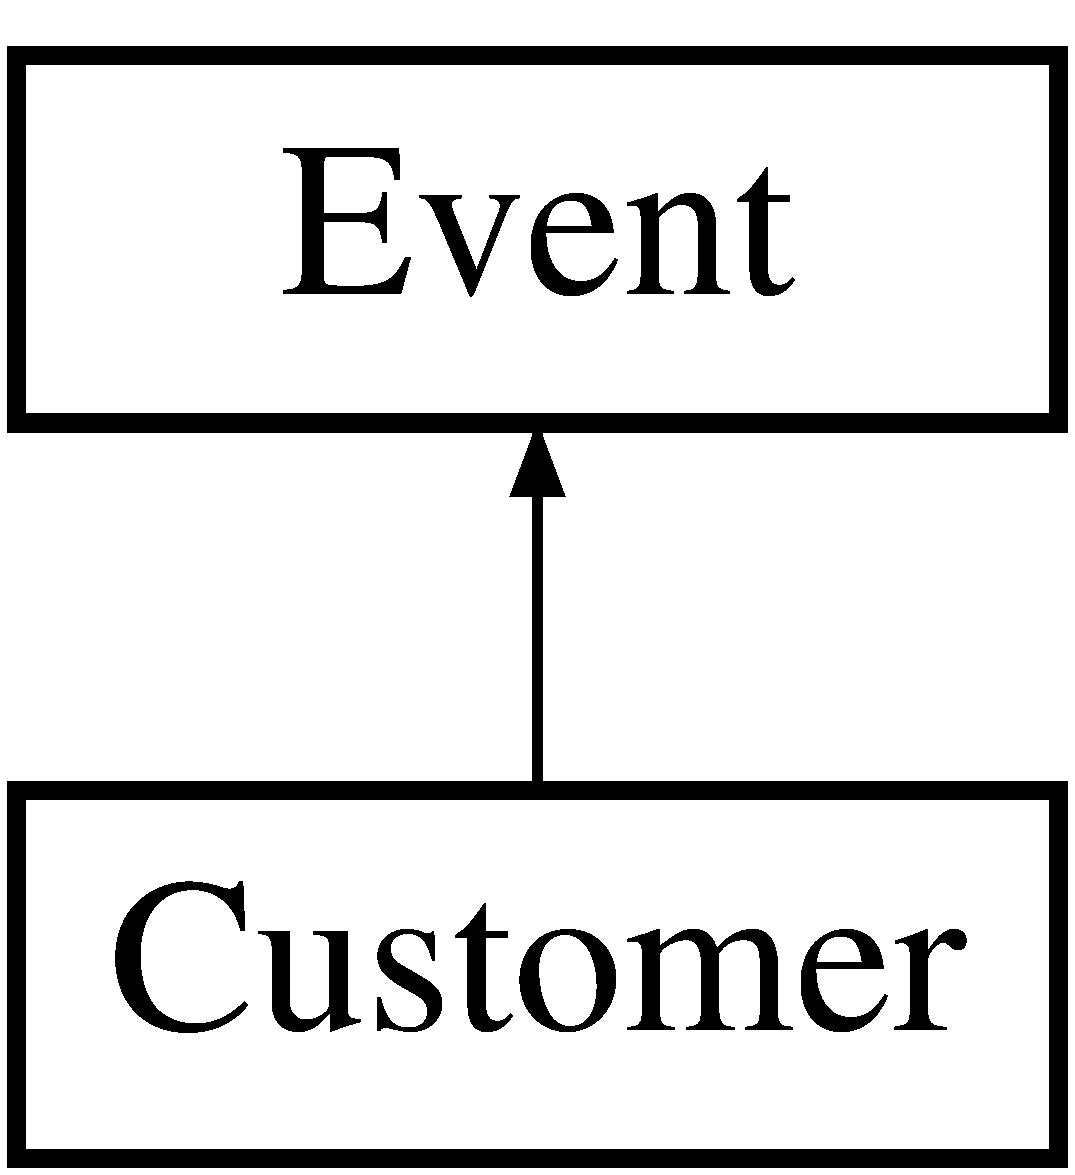
\includegraphics[height=2.000000cm]{classCustomer}
\end{center}
\end{figure}
\subsection*{Public Member Functions}
\begin{DoxyCompactItemize}
\item 
\textbf{ Customer} ()
\item 
\textbf{ Customer} (int \textbf{ t})
\item 
\textbf{ Event} $\ast$ \textbf{ add} ()
\item 
int \textbf{ get\+Time} ()
\item 
void \textbf{ action\+\_\+single\+\_\+line} ()
\item 
void \textbf{ action\+\_\+multiple\+\_\+lines} ()
\item 
virtual \textbf{ $\sim$\+Customer} ()
\end{DoxyCompactItemize}
\subsection*{Public Attributes}
\begin{DoxyCompactItemize}
\item 
int \textbf{ time}
\end{DoxyCompactItemize}


\subsection{Detailed Description}
\doxyref{Customer}{p.}{classCustomer} is a derived \doxyref{Event}{p.}{classEvent} class that contains information on how long a customer was in the bank for. 

\subsection{Constructor \& Destructor Documentation}
\mbox{\label{classCustomer_abcc8fae9701e5ba9d7d6fe44498b34e3}} 
\index{Customer@{Customer}!Customer@{Customer}}
\index{Customer@{Customer}!Customer@{Customer}}
\subsubsection{Customer()\hspace{0.1cm}{\footnotesize\ttfamily [1/2]}}
{\footnotesize\ttfamily Customer\+::\+Customer (\begin{DoxyParamCaption}{ }\end{DoxyParamCaption})\hspace{0.3cm}{\ttfamily [inline]}}

\mbox{\label{classCustomer_ad0509039bdcad60a3ec631b08d904ad3}} 
\index{Customer@{Customer}!Customer@{Customer}}
\index{Customer@{Customer}!Customer@{Customer}}
\subsubsection{Customer()\hspace{0.1cm}{\footnotesize\ttfamily [2/2]}}
{\footnotesize\ttfamily Customer\+::\+Customer (\begin{DoxyParamCaption}\item[{int}]{t }\end{DoxyParamCaption})\hspace{0.3cm}{\ttfamily [inline]}}



References action\+\_\+multiple\+\_\+lines(), action\+\_\+single\+\_\+line(), add(), get\+Time(), and t.

\mbox{\label{classCustomer_a7784915654b180d09696edded3db913d}} 
\index{Customer@{Customer}!````~Customer@{$\sim$\+Customer}}
\index{````~Customer@{$\sim$\+Customer}!Customer@{Customer}}
\subsubsection{$\sim$\+Customer()}
{\footnotesize\ttfamily virtual Customer\+::$\sim$\+Customer (\begin{DoxyParamCaption}{ }\end{DoxyParamCaption})\hspace{0.3cm}{\ttfamily [inline]}, {\ttfamily [virtual]}}



\subsection{Member Function Documentation}
\mbox{\label{classCustomer_a308e99ea9a319588c258096cc7d67619}} 
\index{Customer@{Customer}!action\+\_\+multiple\+\_\+lines@{action\+\_\+multiple\+\_\+lines}}
\index{action\+\_\+multiple\+\_\+lines@{action\+\_\+multiple\+\_\+lines}!Customer@{Customer}}
\subsubsection{action\+\_\+multiple\+\_\+lines()}
{\footnotesize\ttfamily void Customer\+::action\+\_\+multiple\+\_\+lines (\begin{DoxyParamCaption}{ }\end{DoxyParamCaption})\hspace{0.3cm}{\ttfamily [virtual]}}

\doxyref{action\+\_\+multiple\+\_\+lines()}{p.}{classCustomer_a308e99ea9a319588c258096cc7d67619} runs the action for a customer when there are multiple teller queues. this function effectively figures out which line is shortest and adds a customer to that corresponding line if multiple lines have the same length the customer is added to a random line. 

Reimplemented from \textbf{ Event} \doxyref{}{p.}{classEvent_af197959167ba84c6be2f620b32e3b5e5}.



References Event\+Queue\+::add(), customers\+\_\+in\+\_\+line, and tellers.



Referenced by Customer().

\mbox{\label{classCustomer_a36c3b10fb6173b58a47ecbbd940a059d}} 
\index{Customer@{Customer}!action\+\_\+single\+\_\+line@{action\+\_\+single\+\_\+line}}
\index{action\+\_\+single\+\_\+line@{action\+\_\+single\+\_\+line}!Customer@{Customer}}
\subsubsection{action\+\_\+single\+\_\+line()}
{\footnotesize\ttfamily void Customer\+::action\+\_\+single\+\_\+line (\begin{DoxyParamCaption}{ }\end{DoxyParamCaption})\hspace{0.3cm}{\ttfamily [virtual]}}

\doxyref{action\+\_\+single\+\_\+line()}{p.}{classCustomer_a36c3b10fb6173b58a47ecbbd940a059d} performs the action for a customer in a single line simulation according to the guidelines \doxyref{action\+\_\+single\+\_\+line()}{p.}{classCustomer_a36c3b10fb6173b58a47ecbbd940a059d} does as specified in the handout instructions, the first customer in line is taken out and his time is incremented with the idle time of waiting in line. Then the global variables for data being tracked are updated accordingly, such as total\+\_\+idle\+\_\+time and times\+\_\+idle. The customer is then readded to the queue with the updated time. Then a random transaction time is generated for the customer and it is added to his time, and again other global variables are updated, total\+\_\+time and total\+\_\+transaction\+\_\+time get updated. 

Reimplemented from \textbf{ Event} \doxyref{}{p.}{classEvent_a06dcd0b52b9b7dbbf4b43e60702098d7}.



References Event\+Queue\+::add(), Event\+::add\+\_\+time(), avg\+\_\+service\+\_\+time, Event\+Queue\+::front(), Event\+::get\+Idle(), Event\+::get\+Time(), max\+\_\+time\+\_\+until\+\_\+service, Event\+Queue\+::remove(), time\+\_\+in\+\_\+bank, times\+\_\+idle, total\+\_\+idle\+\_\+time, total\+\_\+time, and total\+\_\+transaction\+\_\+time.



Referenced by Customer().

\mbox{\label{classCustomer_a3b442d7e7f188dbf297d750c991f59ee}} 
\index{Customer@{Customer}!add@{add}}
\index{add@{add}!Customer@{Customer}}
\subsubsection{add()}
{\footnotesize\ttfamily \textbf{ Event} $\ast$ Customer\+::add (\begin{DoxyParamCaption}{ }\end{DoxyParamCaption})\hspace{0.3cm}{\ttfamily [virtual]}}

\doxyref{add()}{p.}{classCustomer_a3b442d7e7f188dbf297d750c991f59ee} creates a new \doxyref{Customer}{p.}{classCustomer} event with a random arrival time and returns a pointer to it \doxyref{add()}{p.}{classCustomer_a3b442d7e7f188dbf297d750c991f59ee} generates a random arrival time using the max simulation time from the command line input to create a random time. \begin{DoxyReturn}{Returns}
A pointer to the new customer event created 
\end{DoxyReturn}


Reimplemented from \textbf{ Event} \doxyref{}{p.}{classEvent_a0e9f39799c37a7c676f376cf786e9e58}.



References simulation\+\_\+time.



Referenced by Customer().

\mbox{\label{classCustomer_a34f99014d4f23a474dea0dd337345370}} 
\index{Customer@{Customer}!get\+Time@{get\+Time}}
\index{get\+Time@{get\+Time}!Customer@{Customer}}
\subsubsection{get\+Time()}
{\footnotesize\ttfamily int Customer\+::get\+Time (\begin{DoxyParamCaption}{ }\end{DoxyParamCaption})\hspace{0.3cm}{\ttfamily [virtual]}}

\doxyref{get\+Time()}{p.}{classCustomer_a34f99014d4f23a474dea0dd337345370} returns the arrival time of a customer object

\begin{DoxyReturn}{Returns}
The arrival time of a customer 
\end{DoxyReturn}


Reimplemented from \textbf{ Event} \doxyref{}{p.}{classEvent_a32abdebfd9f3e62bbc7ef36ba7b6964a}.



Referenced by Customer().



\subsection{Member Data Documentation}
\mbox{\label{classCustomer_ad94d570ce65268bba8466928e946fbcf}} 
\index{Customer@{Customer}!time@{time}}
\index{time@{time}!Customer@{Customer}}
\subsubsection{time}
{\footnotesize\ttfamily int Customer\+::time}



The documentation for this class was generated from the following files\+:\begin{DoxyCompactItemize}
\item 
\textbf{ customer.\+h}\item 
\textbf{ customer.\+cpp}\end{DoxyCompactItemize}

\section{Event Class Reference}
\label{classEvent}\index{Event@{Event}}


\doxyref{Event}{p.}{classEvent} is an abstract class that contains the time an event occurs at.  




{\ttfamily \#include $<$event.\+h$>$}

Inheritance diagram for Event\+:\begin{figure}[H]
\begin{center}
\leavevmode
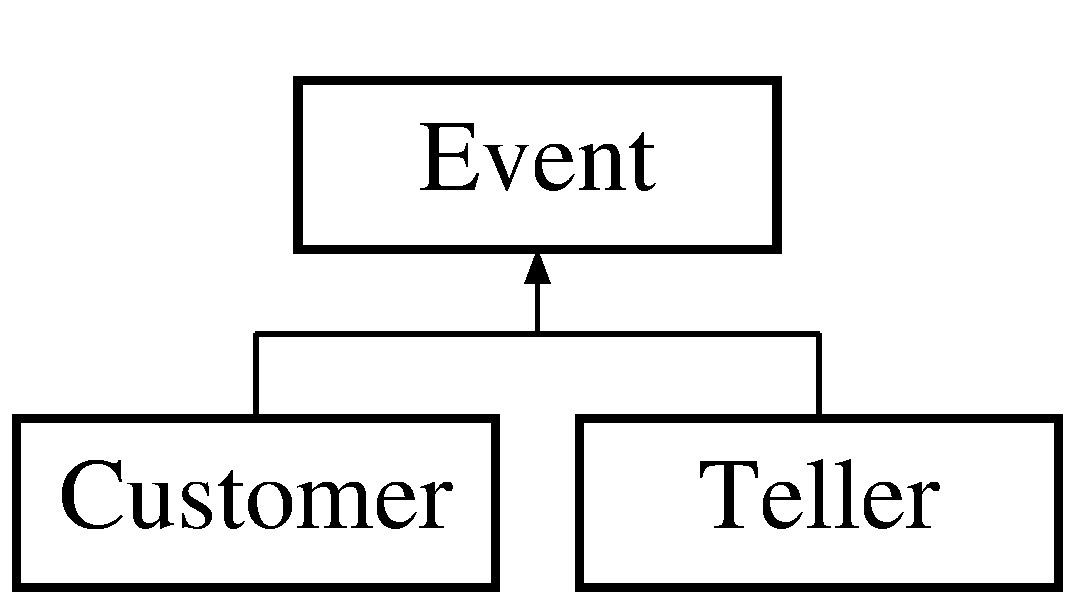
\includegraphics[height=2.000000cm]{classEvent}
\end{center}
\end{figure}
\subsection*{Public Member Functions}
\begin{DoxyCompactItemize}
\item 
\textbf{ Event} ()
\item 
virtual \textbf{ Event} $\ast$ \textbf{ add} ()
\item 
virtual int \textbf{ get\+Time} ()
\item 
virtual int \textbf{ get\+Idle} ()
\item 
virtual void \textbf{ action\+\_\+single\+\_\+line} ()
\item 
virtual void \textbf{ action\+\_\+multiple\+\_\+lines} ()
\item 
virtual void \textbf{ add\+\_\+time} (int transaction\+\_\+time)
\item 
virtual \textbf{ $\sim$\+Event} ()
\end{DoxyCompactItemize}
\subsection*{Public Attributes}
\begin{DoxyCompactItemize}
\item 
int \textbf{ line}
\end{DoxyCompactItemize}


\subsection{Detailed Description}
\doxyref{Event}{p.}{classEvent} is an abstract class that contains the time an event occurs at. 

\subsection{Constructor \& Destructor Documentation}
\mbox{\label{classEvent_a5a40dd4708297f7031e29b39e039ae10}} 
\index{Event@{Event}!Event@{Event}}
\index{Event@{Event}!Event@{Event}}
\subsubsection{Event()}
{\footnotesize\ttfamily Event\+::\+Event (\begin{DoxyParamCaption}{ }\end{DoxyParamCaption})\hspace{0.3cm}{\ttfamily [inline]}}

\mbox{\label{classEvent_ab864fd85c758006c42cd7a1b3369b483}} 
\index{Event@{Event}!````~Event@{$\sim$\+Event}}
\index{````~Event@{$\sim$\+Event}!Event@{Event}}
\subsubsection{$\sim$\+Event()}
{\footnotesize\ttfamily virtual Event\+::$\sim$\+Event (\begin{DoxyParamCaption}{ }\end{DoxyParamCaption})\hspace{0.3cm}{\ttfamily [inline]}, {\ttfamily [virtual]}}



\subsection{Member Function Documentation}
\mbox{\label{classEvent_af197959167ba84c6be2f620b32e3b5e5}} 
\index{Event@{Event}!action\+\_\+multiple\+\_\+lines@{action\+\_\+multiple\+\_\+lines}}
\index{action\+\_\+multiple\+\_\+lines@{action\+\_\+multiple\+\_\+lines}!Event@{Event}}
\subsubsection{action\+\_\+multiple\+\_\+lines()}
{\footnotesize\ttfamily virtual void Event\+::action\+\_\+multiple\+\_\+lines (\begin{DoxyParamCaption}{ }\end{DoxyParamCaption})\hspace{0.3cm}{\ttfamily [inline]}, {\ttfamily [virtual]}}



Reimplemented in \textbf{ Teller} \doxyref{}{p.}{classTeller_a621763217078fffb621648f9ceb662ce}, and \textbf{ Customer} \doxyref{}{p.}{classCustomer_a308e99ea9a319588c258096cc7d67619}.



Referenced by Event\+Queue\+::get\+Next\+Multiple\+Lines().

\mbox{\label{classEvent_a06dcd0b52b9b7dbbf4b43e60702098d7}} 
\index{Event@{Event}!action\+\_\+single\+\_\+line@{action\+\_\+single\+\_\+line}}
\index{action\+\_\+single\+\_\+line@{action\+\_\+single\+\_\+line}!Event@{Event}}
\subsubsection{action\+\_\+single\+\_\+line()}
{\footnotesize\ttfamily virtual void Event\+::action\+\_\+single\+\_\+line (\begin{DoxyParamCaption}{ }\end{DoxyParamCaption})\hspace{0.3cm}{\ttfamily [inline]}, {\ttfamily [virtual]}}



Reimplemented in \textbf{ Teller} \doxyref{}{p.}{classTeller_a343a401c4c129df27bb1cd7d8d04b140}, and \textbf{ Customer} \doxyref{}{p.}{classCustomer_a36c3b10fb6173b58a47ecbbd940a059d}.



Referenced by Event\+Queue\+::get\+Next().

\mbox{\label{classEvent_a0e9f39799c37a7c676f376cf786e9e58}} 
\index{Event@{Event}!add@{add}}
\index{add@{add}!Event@{Event}}
\subsubsection{add()}
{\footnotesize\ttfamily virtual \textbf{ Event}$\ast$ Event\+::add (\begin{DoxyParamCaption}{ }\end{DoxyParamCaption})\hspace{0.3cm}{\ttfamily [inline]}, {\ttfamily [virtual]}}



Reimplemented in \textbf{ Teller} \doxyref{}{p.}{classTeller_a1c45587ecdc913a27fa2ca6b144662d1}, and \textbf{ Customer} \doxyref{}{p.}{classCustomer_a3b442d7e7f188dbf297d750c991f59ee}.



Referenced by sim\+\_\+multiple\+\_\+lines(), and sim\+\_\+single\+\_\+line().

\mbox{\label{classEvent_a272570d4be9af6af85f011808a5cce6e}} 
\index{Event@{Event}!add\+\_\+time@{add\+\_\+time}}
\index{add\+\_\+time@{add\+\_\+time}!Event@{Event}}
\subsubsection{add\+\_\+time()}
{\footnotesize\ttfamily virtual void Event\+::add\+\_\+time (\begin{DoxyParamCaption}\item[{int}]{transaction\+\_\+time }\end{DoxyParamCaption})\hspace{0.3cm}{\ttfamily [inline]}, {\ttfamily [virtual]}}



Reimplemented in \textbf{ Teller} \doxyref{}{p.}{classTeller_ab61ca608447bbe7510407461126f5e18}.



Referenced by Customer\+::action\+\_\+single\+\_\+line().

\mbox{\label{classEvent_a9cade0f8d2c601413bfe8e9ec0a11735}} 
\index{Event@{Event}!get\+Idle@{get\+Idle}}
\index{get\+Idle@{get\+Idle}!Event@{Event}}
\subsubsection{get\+Idle()}
{\footnotesize\ttfamily virtual int Event\+::get\+Idle (\begin{DoxyParamCaption}{ }\end{DoxyParamCaption})\hspace{0.3cm}{\ttfamily [inline]}, {\ttfamily [virtual]}}



Reimplemented in \textbf{ Teller} \doxyref{}{p.}{classTeller_a887f25b29989b3e60a003b113acf4d48}.



Referenced by Customer\+::action\+\_\+single\+\_\+line().

\mbox{\label{classEvent_a32abdebfd9f3e62bbc7ef36ba7b6964a}} 
\index{Event@{Event}!get\+Time@{get\+Time}}
\index{get\+Time@{get\+Time}!Event@{Event}}
\subsubsection{get\+Time()}
{\footnotesize\ttfamily virtual int Event\+::get\+Time (\begin{DoxyParamCaption}{ }\end{DoxyParamCaption})\hspace{0.3cm}{\ttfamily [inline]}, {\ttfamily [virtual]}}



Reimplemented in \textbf{ Teller} \doxyref{}{p.}{classTeller_a2911d4ddbe6548083c7df6face642532}, and \textbf{ Customer} \doxyref{}{p.}{classCustomer_a34f99014d4f23a474dea0dd337345370}.



Referenced by Customer\+::action\+\_\+single\+\_\+line(), Compare\+Events\+::operator()(), and Teller\+::process\+\_\+transaction().



\subsection{Member Data Documentation}
\mbox{\label{classEvent_a9a3b4e3b3e3c38d71bfe8ffa5e841782}} 
\index{Event@{Event}!line@{line}}
\index{line@{line}!Event@{Event}}
\subsubsection{line}
{\footnotesize\ttfamily int Event\+::line}



Referenced by sim\+\_\+multiple\+\_\+lines().



The documentation for this class was generated from the following file\+:\begin{DoxyCompactItemize}
\item 
\textbf{ event.\+h}\end{DoxyCompactItemize}

\section{Event\+Queue Class Reference}
\label{classEventQueue}\index{Event\+Queue@{Event\+Queue}}


\doxyref{Event\+Queue}{p.}{classEventQueue} is a priorty\+\_\+queue of events, is the global overhead for the entire project.  




{\ttfamily \#include $<$eventqueue.\+h$>$}

Inheritance diagram for Event\+Queue\+:\begin{figure}[H]
\begin{center}
\leavevmode
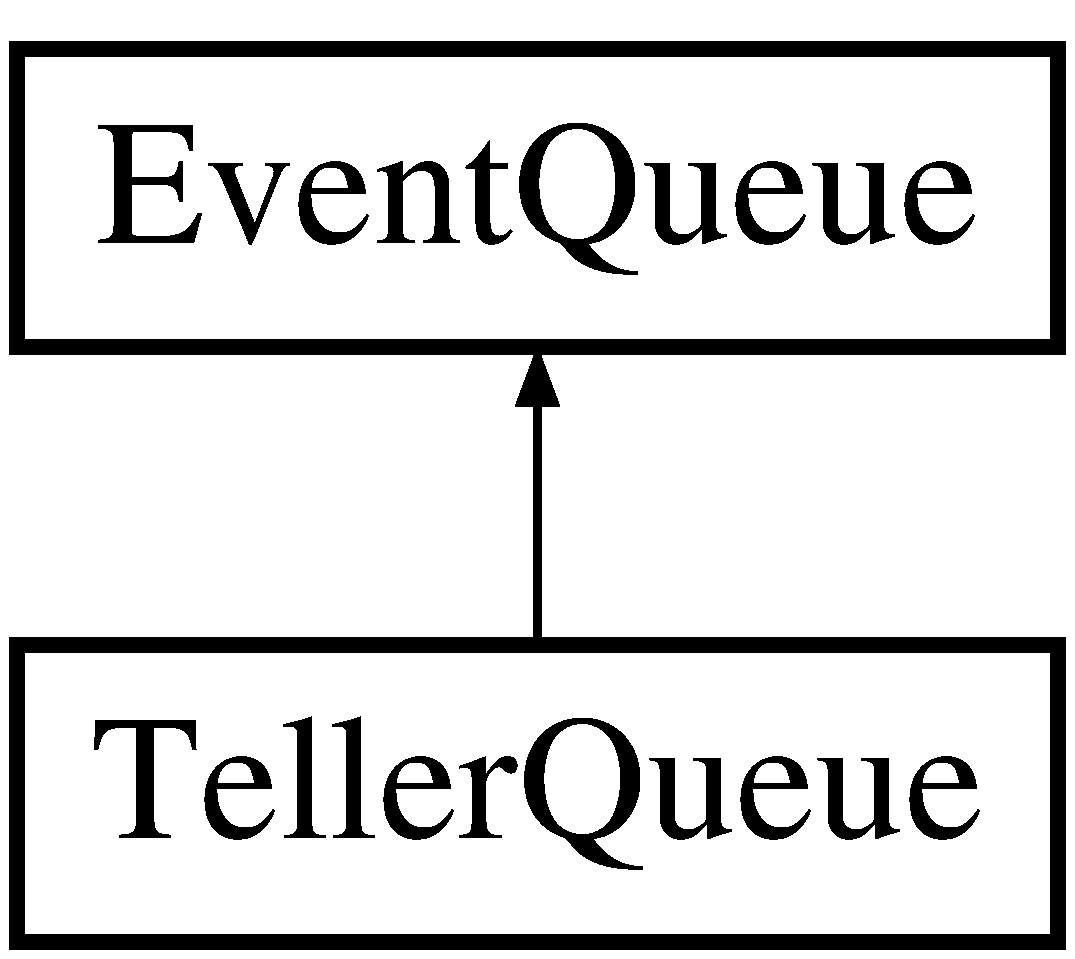
\includegraphics[height=2.000000cm]{classEventQueue}
\end{center}
\end{figure}
\subsection*{Public Member Functions}
\begin{DoxyCompactItemize}
\item 
\textbf{ Event\+Queue} ()
\item 
void \textbf{ get\+Next} ()
\item 
void \textbf{ get\+Next\+Multiple\+Lines} ()
\item 
\textbf{ Event} $\ast$ \textbf{ front} ()
\item 
void \textbf{ remove} ()
\item 
void \textbf{ add} (\textbf{ Event} $\ast$a)
\end{DoxyCompactItemize}
\subsection*{Public Attributes}
\begin{DoxyCompactItemize}
\item 
std\+::priority\+\_\+queue$<$ \textbf{ Event} $\ast$, std\+::vector$<$ \textbf{ Event} $\ast$ $>$, \textbf{ Compare\+Events} $>$ \textbf{ eq}
\end{DoxyCompactItemize}


\subsection{Detailed Description}
\doxyref{Event\+Queue}{p.}{classEventQueue} is a priorty\+\_\+queue of events, is the global overhead for the entire project. 

\subsection{Constructor \& Destructor Documentation}
\mbox{\label{classEventQueue_ab7de5a41befc94aac0f461391e67f14a}} 
\index{Event\+Queue@{Event\+Queue}!Event\+Queue@{Event\+Queue}}
\index{Event\+Queue@{Event\+Queue}!Event\+Queue@{Event\+Queue}}
\subsubsection{Event\+Queue()}
{\footnotesize\ttfamily Event\+Queue\+::\+Event\+Queue (\begin{DoxyParamCaption}{ }\end{DoxyParamCaption})\hspace{0.3cm}{\ttfamily [inline]}}



\subsection{Member Function Documentation}
\mbox{\label{classEventQueue_a9a0105eb1a4798cd5b5064c94f7d0954}} 
\index{Event\+Queue@{Event\+Queue}!add@{add}}
\index{add@{add}!Event\+Queue@{Event\+Queue}}
\subsubsection{add()}
{\footnotesize\ttfamily void Event\+Queue\+::add (\begin{DoxyParamCaption}\item[{\textbf{ Event} $\ast$}]{event }\end{DoxyParamCaption})}

\doxyref{add()}{p.}{classEventQueue_a9a0105eb1a4798cd5b5064c94f7d0954} takes a pointer to an event and adds it to the queue 

References eq.



Referenced by Customer\+::action\+\_\+multiple\+\_\+lines(), Teller\+::action\+\_\+multiple\+\_\+lines(), Customer\+::action\+\_\+single\+\_\+line(), Teller\+::process\+\_\+transaction(), sim\+\_\+multiple\+\_\+lines(), and sim\+\_\+single\+\_\+line().

\mbox{\label{classEventQueue_ae8ca507accdf109bc487034b299d0f62}} 
\index{Event\+Queue@{Event\+Queue}!front@{front}}
\index{front@{front}!Event\+Queue@{Event\+Queue}}
\subsubsection{front()}
{\footnotesize\ttfamily \textbf{ Event} $\ast$ Event\+Queue\+::front (\begin{DoxyParamCaption}{ }\end{DoxyParamCaption})}

\doxyref{front()}{p.}{classEventQueue_ae8ca507accdf109bc487034b299d0f62} returns a pointer to the first element in the queue \begin{DoxyReturn}{Returns}
a pointer to the first \doxyref{Event}{p.}{classEvent} in the queue 
\end{DoxyReturn}


References eq.



Referenced by Customer\+::action\+\_\+single\+\_\+line(), and Teller\+::process\+\_\+transaction().

\mbox{\label{classEventQueue_a4caa21498f84ed469d39cb0b9e0e6dd0}} 
\index{Event\+Queue@{Event\+Queue}!get\+Next@{get\+Next}}
\index{get\+Next@{get\+Next}!Event\+Queue@{Event\+Queue}}
\subsubsection{get\+Next()}
{\footnotesize\ttfamily void Event\+Queue\+::get\+Next (\begin{DoxyParamCaption}{ }\end{DoxyParamCaption})}

\doxyref{get\+Next()}{p.}{classEventQueue_a4caa21498f84ed469d39cb0b9e0e6dd0} removes the first event in the queue and runs the action for it \doxyref{get\+Next()}{p.}{classEventQueue_a4caa21498f84ed469d39cb0b9e0e6dd0} takes off the first event and runs the corresponding event, either customer or teller, this function is used for a one line simulation 

References Event\+::action\+\_\+single\+\_\+line(), and eq.



Referenced by sim\+\_\+single\+\_\+line().

\mbox{\label{classEventQueue_a3af432f6e5af6071c3eeb13d16c1288d}} 
\index{Event\+Queue@{Event\+Queue}!get\+Next\+Multiple\+Lines@{get\+Next\+Multiple\+Lines}}
\index{get\+Next\+Multiple\+Lines@{get\+Next\+Multiple\+Lines}!Event\+Queue@{Event\+Queue}}
\subsubsection{get\+Next\+Multiple\+Lines()}
{\footnotesize\ttfamily void Event\+Queue\+::get\+Next\+Multiple\+Lines (\begin{DoxyParamCaption}{ }\end{DoxyParamCaption})}

\doxyref{get\+Next\+Multiple\+Lines()}{p.}{classEventQueue_a3af432f6e5af6071c3eeb13d16c1288d} takes the first event off the queue and runs the action for it, for multiple lines does the same as \doxyref{get\+Next()}{p.}{classEventQueue_a4caa21498f84ed469d39cb0b9e0e6dd0} function, but used for multiple line simulation instead 

References Event\+::action\+\_\+multiple\+\_\+lines(), and eq.



Referenced by sim\+\_\+multiple\+\_\+lines().

\mbox{\label{classEventQueue_a81f74630368648a1dd6d8ee2656fda75}} 
\index{Event\+Queue@{Event\+Queue}!remove@{remove}}
\index{remove@{remove}!Event\+Queue@{Event\+Queue}}
\subsubsection{remove()}
{\footnotesize\ttfamily void Event\+Queue\+::remove (\begin{DoxyParamCaption}{ }\end{DoxyParamCaption})}

\doxyref{remove()}{p.}{classEventQueue_a81f74630368648a1dd6d8ee2656fda75} removes the first element from the queue 

References eq.



Referenced by Customer\+::action\+\_\+single\+\_\+line(), and Teller\+::process\+\_\+transaction().



\subsection{Member Data Documentation}
\mbox{\label{classEventQueue_a4e9008a24e40e43b72ad1d72d57b8d67}} 
\index{Event\+Queue@{Event\+Queue}!eq@{eq}}
\index{eq@{eq}!Event\+Queue@{Event\+Queue}}
\subsubsection{eq}
{\footnotesize\ttfamily std\+::priority\+\_\+queue$<$\textbf{ Event} $\ast$, std\+::vector$<$\textbf{ Event} $\ast$$>$, \textbf{ Compare\+Events}$>$ Event\+Queue\+::eq}



Referenced by Teller\+::action\+\_\+single\+\_\+line(), add(), front(), get\+Next(), get\+Next\+Multiple\+Lines(), remove(), sim\+\_\+multiple\+\_\+lines(), and sim\+\_\+single\+\_\+line().



The documentation for this class was generated from the following files\+:\begin{DoxyCompactItemize}
\item 
\textbf{ eventqueue.\+h}\item 
\textbf{ eventqueue.\+cpp}\end{DoxyCompactItemize}

\section{Teller Class Reference}
\label{classTeller}\index{Teller@{Teller}}


\doxyref{Teller}{p.}{classTeller} is the derived class of \doxyref{Event}{p.}{classEvent} that carries additional info such as idle\+\_\+time for each specific teller.  




{\ttfamily \#include $<$teller.\+h$>$}

Inheritance diagram for Teller\+:\begin{figure}[H]
\begin{center}
\leavevmode
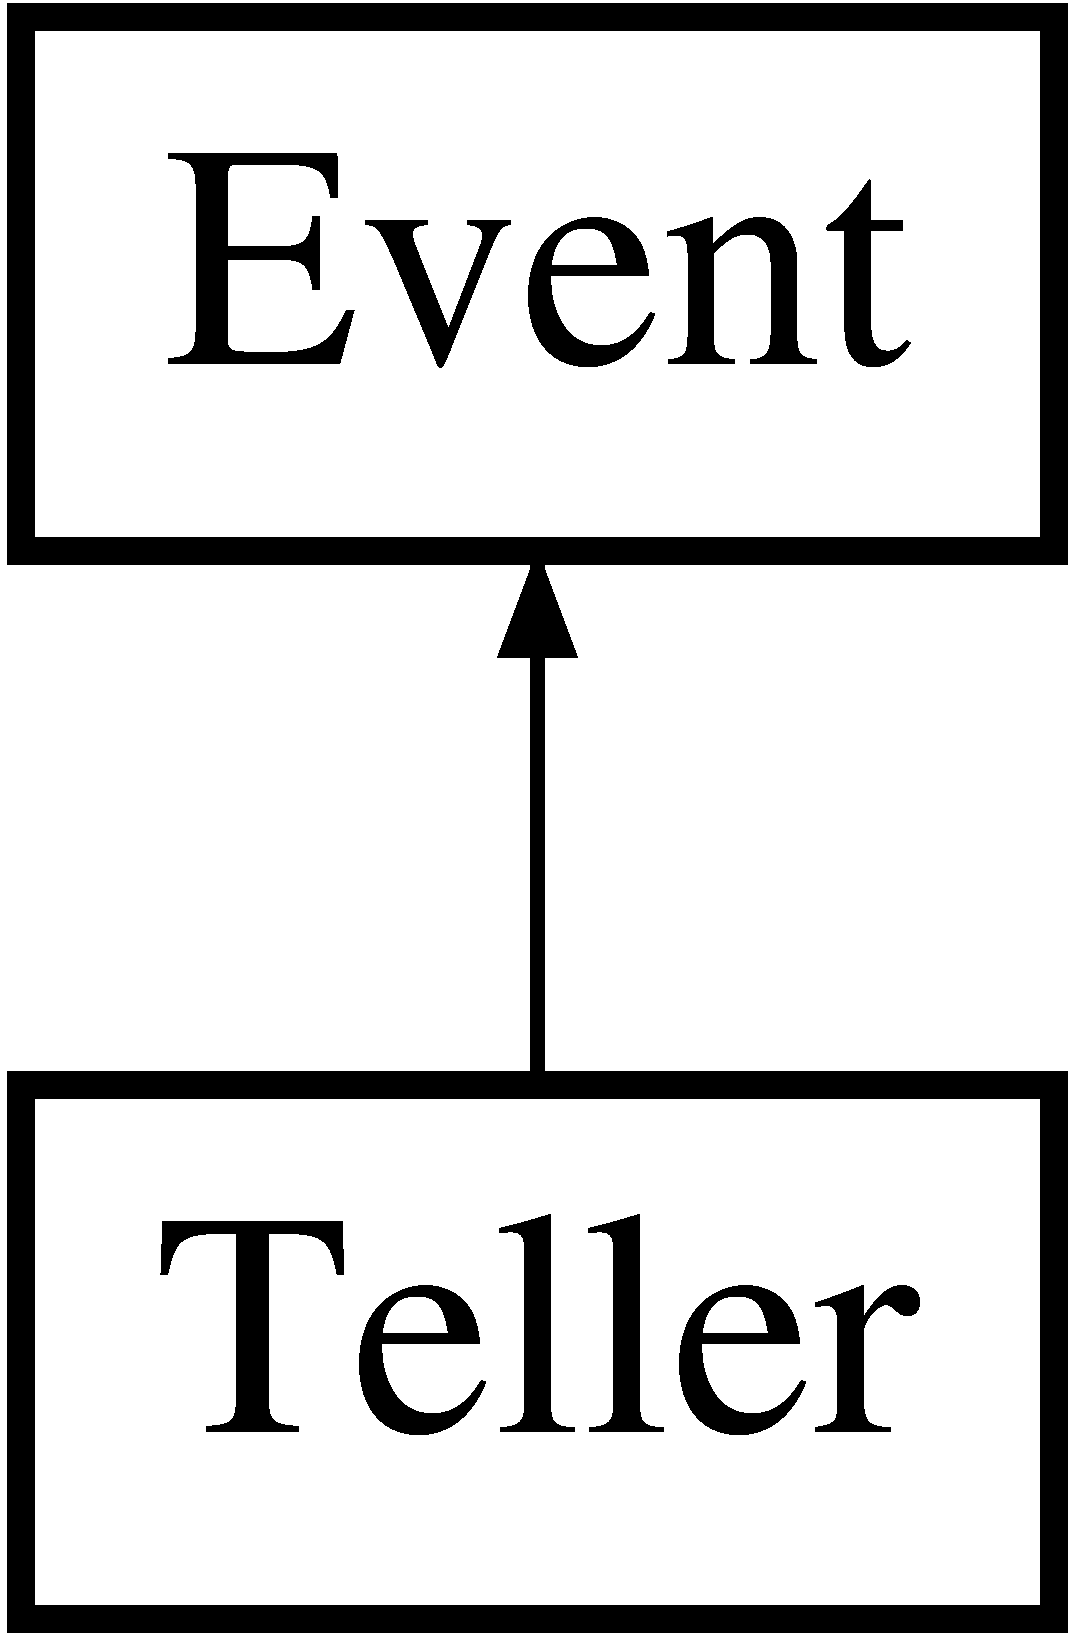
\includegraphics[height=2.000000cm]{classTeller}
\end{center}
\end{figure}
\subsection*{Public Member Functions}
\begin{DoxyCompactItemize}
\item 
\textbf{ Teller} ()
\item 
\textbf{ Teller} (int idle\+\_\+t)
\item 
\textbf{ Event} $\ast$ \textbf{ add} ()
\item 
int \textbf{ get\+Time} ()
\item 
int \textbf{ get\+Idle} ()
\item 
void \textbf{ action\+\_\+single\+\_\+line} ()
\item 
void \textbf{ action\+\_\+multiple\+\_\+lines} ()
\item 
void \textbf{ add\+\_\+time} (int transaction\+\_\+time)
\item 
void \textbf{ process\+\_\+transaction} (int line\+\_\+number)
\item 
virtual \textbf{ $\sim$\+Teller} ()
\end{DoxyCompactItemize}
\subsection*{Public Attributes}
\begin{DoxyCompactItemize}
\item 
int \textbf{ idle\+\_\+time}
\item 
int \textbf{ time}
\end{DoxyCompactItemize}


\subsection{Detailed Description}
\doxyref{Teller}{p.}{classTeller} is the derived class of \doxyref{Event}{p.}{classEvent} that carries additional info such as idle\+\_\+time for each specific teller. 

\subsection{Constructor \& Destructor Documentation}
\mbox{\label{classTeller_a652e56e65d8d73a53d709b8299e1c4a7}} 
\index{Teller@{Teller}!Teller@{Teller}}
\index{Teller@{Teller}!Teller@{Teller}}
\subsubsection{Teller()\hspace{0.1cm}{\footnotesize\ttfamily [1/2]}}
{\footnotesize\ttfamily Teller\+::\+Teller (\begin{DoxyParamCaption}{ }\end{DoxyParamCaption})\hspace{0.3cm}{\ttfamily [inline]}}

\mbox{\label{classTeller_a1a91a9848e1bbf11fc7552bc26e63842}} 
\index{Teller@{Teller}!Teller@{Teller}}
\index{Teller@{Teller}!Teller@{Teller}}
\subsubsection{Teller()\hspace{0.1cm}{\footnotesize\ttfamily [2/2]}}
{\footnotesize\ttfamily Teller\+::\+Teller (\begin{DoxyParamCaption}\item[{int}]{idle\+\_\+t }\end{DoxyParamCaption})\hspace{0.3cm}{\ttfamily [inline]}}



References action\+\_\+multiple\+\_\+lines(), action\+\_\+single\+\_\+line(), add(), add\+\_\+time(), get\+Idle(), get\+Time(), and process\+\_\+transaction().

\mbox{\label{classTeller_ac4c2dd4ecf85d90691cdfb77d5f61bd6}} 
\index{Teller@{Teller}!````~Teller@{$\sim$\+Teller}}
\index{````~Teller@{$\sim$\+Teller}!Teller@{Teller}}
\subsubsection{$\sim$\+Teller()}
{\footnotesize\ttfamily virtual Teller\+::$\sim$\+Teller (\begin{DoxyParamCaption}{ }\end{DoxyParamCaption})\hspace{0.3cm}{\ttfamily [inline]}, {\ttfamily [virtual]}}



\subsection{Member Function Documentation}
\mbox{\label{classTeller_a621763217078fffb621648f9ceb662ce}} 
\index{Teller@{Teller}!action\+\_\+multiple\+\_\+lines@{action\+\_\+multiple\+\_\+lines}}
\index{action\+\_\+multiple\+\_\+lines@{action\+\_\+multiple\+\_\+lines}!Teller@{Teller}}
\subsubsection{action\+\_\+multiple\+\_\+lines()}
{\footnotesize\ttfamily void Teller\+::action\+\_\+multiple\+\_\+lines (\begin{DoxyParamCaption}{ }\end{DoxyParamCaption})\hspace{0.3cm}{\ttfamily [virtual]}}

\doxyref{action\+\_\+multiple\+\_\+lines()}{p.}{classTeller_a621763217078fffb621648f9ceb662ce} either helps a customers or goes idle adds a teller event to the event queue with idle time, or processes a transaction for a customer in the tellers line, if not the teller looks to other lines to see if anyone needs help and if no one does goes idle. 

Reimplemented from \textbf{ Event} \doxyref{}{p.}{classEvent_af197959167ba84c6be2f620b32e3b5e5}.



References Event\+Queue\+::add(), customers\+\_\+in\+\_\+line, max\+\_\+idle\+\_\+time\+\_\+back\+\_\+in\+\_\+queue, min\+\_\+idle\+\_\+time\+\_\+back\+\_\+in\+\_\+queue, simulation\+\_\+time, tellers, time\+\_\+in\+\_\+bank, times\+\_\+idle, and total\+\_\+idle\+\_\+time.



Referenced by Teller().

\mbox{\label{classTeller_a343a401c4c129df27bb1cd7d8d04b140}} 
\index{Teller@{Teller}!action\+\_\+single\+\_\+line@{action\+\_\+single\+\_\+line}}
\index{action\+\_\+single\+\_\+line@{action\+\_\+single\+\_\+line}!Teller@{Teller}}
\subsubsection{action\+\_\+single\+\_\+line()}
{\footnotesize\ttfamily void Teller\+::action\+\_\+single\+\_\+line (\begin{DoxyParamCaption}{ }\end{DoxyParamCaption})\hspace{0.3cm}{\ttfamily [virtual]}}

\doxyref{action\+\_\+single\+\_\+line()}{p.}{classTeller_a343a401c4c129df27bb1cd7d8d04b140} adds this teller event to a teller\+\_\+queue using the add function of the event queue class 

Reimplemented from \textbf{ Event} \doxyref{}{p.}{classEvent_a06dcd0b52b9b7dbbf4b43e60702098d7}.



References Event\+Queue\+::eq.



Referenced by Teller().

\mbox{\label{classTeller_a1c45587ecdc913a27fa2ca6b144662d1}} 
\index{Teller@{Teller}!add@{add}}
\index{add@{add}!Teller@{Teller}}
\subsubsection{add()}
{\footnotesize\ttfamily \textbf{ Event} $\ast$ Teller\+::add (\begin{DoxyParamCaption}{ }\end{DoxyParamCaption})\hspace{0.3cm}{\ttfamily [virtual]}}

\doxyref{add()}{p.}{classTeller_a1c45587ecdc913a27fa2ca6b144662d1} creates a new teller object \doxyref{add()}{p.}{classTeller_a1c45587ecdc913a27fa2ca6b144662d1} creates a new teller object with a random idle time between the min and max, which are 0 to 5 minutes \begin{DoxyReturn}{Returns}
a pointer to the new teller object 
\end{DoxyReturn}


Reimplemented from \textbf{ Event} \doxyref{}{p.}{classEvent_a0e9f39799c37a7c676f376cf786e9e58}.



References max\+\_\+idle\+\_\+time, and min\+\_\+idle\+\_\+time.



Referenced by Teller().

\mbox{\label{classTeller_ab61ca608447bbe7510407461126f5e18}} 
\index{Teller@{Teller}!add\+\_\+time@{add\+\_\+time}}
\index{add\+\_\+time@{add\+\_\+time}!Teller@{Teller}}
\subsubsection{add\+\_\+time()}
{\footnotesize\ttfamily void Teller\+::add\+\_\+time (\begin{DoxyParamCaption}\item[{int}]{transaction\+\_\+time }\end{DoxyParamCaption})\hspace{0.3cm}{\ttfamily [virtual]}}

\doxyref{add\+\_\+time()}{p.}{classTeller_ab61ca608447bbe7510407461126f5e18} adds the transaction\+\_\+time to the time of the teller 
\begin{DoxyParams}{Parameters}
{\em transaction\+\_\+time} & the time to be added to the teller\textquotesingle{}s total time \\
\hline
\end{DoxyParams}


Reimplemented from \textbf{ Event} \doxyref{}{p.}{classEvent_a272570d4be9af6af85f011808a5cce6e}.



Referenced by Teller().

\mbox{\label{classTeller_a887f25b29989b3e60a003b113acf4d48}} 
\index{Teller@{Teller}!get\+Idle@{get\+Idle}}
\index{get\+Idle@{get\+Idle}!Teller@{Teller}}
\subsubsection{get\+Idle()}
{\footnotesize\ttfamily int Teller\+::get\+Idle (\begin{DoxyParamCaption}{ }\end{DoxyParamCaption})\hspace{0.3cm}{\ttfamily [virtual]}}

\doxyref{get\+Idle()}{p.}{classTeller_a887f25b29989b3e60a003b113acf4d48} returns the idle time of a teller object \begin{DoxyReturn}{Returns}
the idle time of a teller object 
\end{DoxyReturn}


Reimplemented from \textbf{ Event} \doxyref{}{p.}{classEvent_a9cade0f8d2c601413bfe8e9ec0a11735}.



Referenced by Teller().

\mbox{\label{classTeller_a2911d4ddbe6548083c7df6face642532}} 
\index{Teller@{Teller}!get\+Time@{get\+Time}}
\index{get\+Time@{get\+Time}!Teller@{Teller}}
\subsubsection{get\+Time()}
{\footnotesize\ttfamily int Teller\+::get\+Time (\begin{DoxyParamCaption}{ }\end{DoxyParamCaption})\hspace{0.3cm}{\ttfamily [virtual]}}

\doxyref{get\+Time()}{p.}{classTeller_a2911d4ddbe6548083c7df6face642532} returns the time of a teller object \begin{DoxyReturn}{Returns}
the time of a teller object 
\end{DoxyReturn}


Reimplemented from \textbf{ Event} \doxyref{}{p.}{classEvent_a32abdebfd9f3e62bbc7ef36ba7b6964a}.



Referenced by Teller().

\mbox{\label{classTeller_aab579ac83fd6337998b96397fb140a55}} 
\index{Teller@{Teller}!process\+\_\+transaction@{process\+\_\+transaction}}
\index{process\+\_\+transaction@{process\+\_\+transaction}!Teller@{Teller}}
\subsubsection{process\+\_\+transaction()}
{\footnotesize\ttfamily void Teller\+::process\+\_\+transaction (\begin{DoxyParamCaption}\item[{int}]{line\+\_\+number }\end{DoxyParamCaption})}

\doxyref{process\+\_\+transaction()}{p.}{classTeller_aab579ac83fd6337998b96397fb140a55} processes a transaction for a specific line passed by input process\+\_\+transaction removes the first event from a teller queue, and generates a random service time, adds it to the customers time and updates globals and readds the teller to the event queue. The customer is not readded as he is done in the bank. 

References Event\+Queue\+::add(), avg\+\_\+service\+\_\+time, customers\+\_\+in\+\_\+line, Event\+Queue\+::front(), Event\+::get\+Time(), Event\+Queue\+::remove(), total\+\_\+time, and total\+\_\+transaction\+\_\+time.



Referenced by Teller().



\subsection{Member Data Documentation}
\mbox{\label{classTeller_ae122728a1f7931206860f28541041516}} 
\index{Teller@{Teller}!idle\+\_\+time@{idle\+\_\+time}}
\index{idle\+\_\+time@{idle\+\_\+time}!Teller@{Teller}}
\subsubsection{idle\+\_\+time}
{\footnotesize\ttfamily int Teller\+::idle\+\_\+time}

\mbox{\label{classTeller_a91b8d3bf984c0bd67d6642df7fe6391f}} 
\index{Teller@{Teller}!time@{time}}
\index{time@{time}!Teller@{Teller}}
\subsubsection{time}
{\footnotesize\ttfamily int Teller\+::time}



The documentation for this class was generated from the following files\+:\begin{DoxyCompactItemize}
\item 
\textbf{ teller.\+h}\item 
\textbf{ teller.\+cpp}\end{DoxyCompactItemize}

\section{Teller\+Queue Class Reference}
\label{classTellerQueue}\index{Teller\+Queue@{Teller\+Queue}}


\doxyref{Teller\+Queue}{p.}{classTellerQueue} is a derived class from \doxyref{Event\+Queue}{p.}{classEventQueue} that does nothing extra, it only holds \doxyref{Customer}{p.}{classCustomer} objects though.  




{\ttfamily \#include $<$teller.\+h$>$}

Inheritance diagram for Teller\+Queue\+:\begin{figure}[H]
\begin{center}
\leavevmode
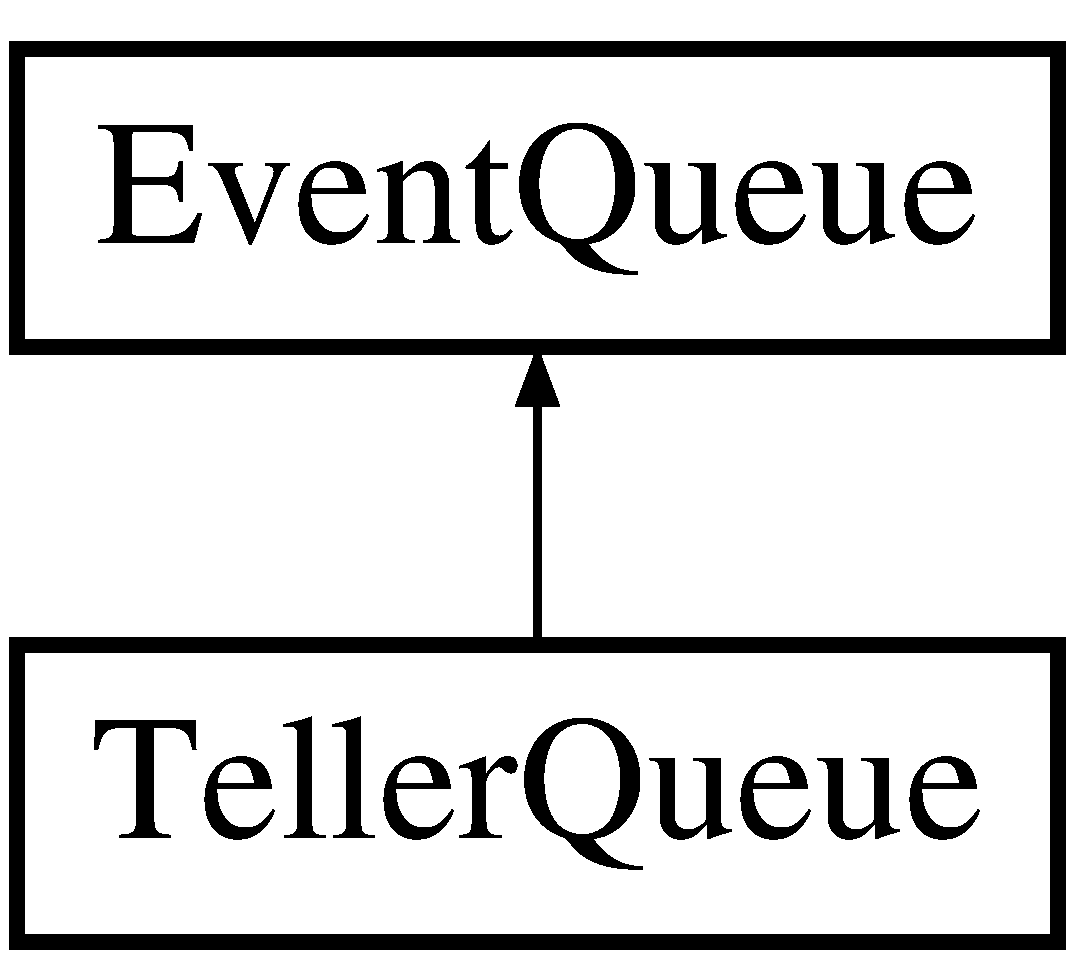
\includegraphics[height=2.000000cm]{classTellerQueue}
\end{center}
\end{figure}
\subsection*{Public Member Functions}
\begin{DoxyCompactItemize}
\item 
\textbf{ Teller\+Queue} ()
\end{DoxyCompactItemize}
\subsection*{Additional Inherited Members}


\subsection{Detailed Description}
\doxyref{Teller\+Queue}{p.}{classTellerQueue} is a derived class from \doxyref{Event\+Queue}{p.}{classEventQueue} that does nothing extra, it only holds \doxyref{Customer}{p.}{classCustomer} objects though. 

\subsection{Constructor \& Destructor Documentation}
\mbox{\label{classTellerQueue_a11d0c867f834ac7a2215013cea9d68fe}} 
\index{Teller\+Queue@{Teller\+Queue}!Teller\+Queue@{Teller\+Queue}}
\index{Teller\+Queue@{Teller\+Queue}!Teller\+Queue@{Teller\+Queue}}
\subsubsection{Teller\+Queue()}
{\footnotesize\ttfamily Teller\+Queue\+::\+Teller\+Queue (\begin{DoxyParamCaption}{ }\end{DoxyParamCaption})\hspace{0.3cm}{\ttfamily [inline]}}



The documentation for this class was generated from the following file\+:\begin{DoxyCompactItemize}
\item 
\textbf{ teller.\+h}\end{DoxyCompactItemize}

\chapter{File Documentation}
\section{customer.\+cpp File Reference}
\label{customer_8cpp}\index{customer.\+cpp@{customer.\+cpp}}
{\ttfamily \#include $<$stdio.\+h$>$}\newline
{\ttfamily \#include $<$stdlib.\+h$>$}\newline
{\ttfamily \#include $<$iostream$>$}\newline
{\ttfamily \#include $<$cstdlib$>$}\newline
{\ttfamily \#include $<$list$>$}\newline
{\ttfamily \#include \char`\"{}sim.\+h\char`\"{}}\newline
{\ttfamily \#include \char`\"{}customer.\+h\char`\"{}}\newline
{\ttfamily \#include \char`\"{}teller.\+h\char`\"{}}\newline
{\ttfamily \#include \char`\"{}event.\+h\char`\"{}}\newline
{\ttfamily \#include \char`\"{}eventqueue.\+h\char`\"{}}\newline
\subsection*{Variables}
\begin{DoxyCompactItemize}
\item 
float \textbf{ simulation\+\_\+time}
\item 
float \textbf{ avg\+\_\+service\+\_\+time}
\item 
int \textbf{ total\+\_\+time}
\item 
int \textbf{ total\+\_\+idle\+\_\+time}
\item 
int \textbf{ times\+\_\+idle}
\item 
int \textbf{ total\+\_\+transaction\+\_\+time}
\item 
int \textbf{ tellers}
\item 
double \textbf{ max\+\_\+time\+\_\+until\+\_\+service}
\item 
int $\ast$ \textbf{ customers\+\_\+in\+\_\+line}
\item 
list$<$ int $>$ \textbf{ time\+\_\+in\+\_\+bank}
\item 
\textbf{ Teller\+Queue} \textbf{ teller\+\_\+queue}
\item 
\textbf{ Teller\+Queue} $\ast$ \textbf{ teller\+\_\+queues}
\end{DoxyCompactItemize}


\subsection{Variable Documentation}
\mbox{\label{customer_8cpp_a210f77aba17cfc74d1447f45e99be1bd}} 
\index{customer.\+cpp@{customer.\+cpp}!avg\+\_\+service\+\_\+time@{avg\+\_\+service\+\_\+time}}
\index{avg\+\_\+service\+\_\+time@{avg\+\_\+service\+\_\+time}!customer.\+cpp@{customer.\+cpp}}
\subsubsection{avg\+\_\+service\+\_\+time}
{\footnotesize\ttfamily float avg\+\_\+service\+\_\+time}



Referenced by Customer\+::action\+\_\+single\+\_\+line().

\mbox{\label{customer_8cpp_abf7392d380d62115dbe6c7c4d74dab62}} 
\index{customer.\+cpp@{customer.\+cpp}!customers\+\_\+in\+\_\+line@{customers\+\_\+in\+\_\+line}}
\index{customers\+\_\+in\+\_\+line@{customers\+\_\+in\+\_\+line}!customer.\+cpp@{customer.\+cpp}}
\subsubsection{customers\+\_\+in\+\_\+line}
{\footnotesize\ttfamily int$\ast$ customers\+\_\+in\+\_\+line}



Referenced by Customer\+::action\+\_\+multiple\+\_\+lines().

\mbox{\label{customer_8cpp_a3babb2af3de98aeed6448910925019dc}} 
\index{customer.\+cpp@{customer.\+cpp}!max\+\_\+time\+\_\+until\+\_\+service@{max\+\_\+time\+\_\+until\+\_\+service}}
\index{max\+\_\+time\+\_\+until\+\_\+service@{max\+\_\+time\+\_\+until\+\_\+service}!customer.\+cpp@{customer.\+cpp}}
\subsubsection{max\+\_\+time\+\_\+until\+\_\+service}
{\footnotesize\ttfamily double max\+\_\+time\+\_\+until\+\_\+service}



Referenced by Customer\+::action\+\_\+single\+\_\+line(), and print().

\mbox{\label{customer_8cpp_a68868698f39e24d72046de64a0adbc70}} 
\index{customer.\+cpp@{customer.\+cpp}!simulation\+\_\+time@{simulation\+\_\+time}}
\index{simulation\+\_\+time@{simulation\+\_\+time}!customer.\+cpp@{customer.\+cpp}}
\subsubsection{simulation\+\_\+time}
{\footnotesize\ttfamily float simulation\+\_\+time}



Referenced by Customer\+::add().

\mbox{\label{customer_8cpp_abf47d44d813ba82d16ab2770fb3f66f4}} 
\index{customer.\+cpp@{customer.\+cpp}!teller\+\_\+queue@{teller\+\_\+queue}}
\index{teller\+\_\+queue@{teller\+\_\+queue}!customer.\+cpp@{customer.\+cpp}}
\subsubsection{teller\+\_\+queue}
{\footnotesize\ttfamily \textbf{ Teller\+Queue} teller\+\_\+queue}

\mbox{\label{customer_8cpp_a0b4f543de738e99fd64f58bb708e2233}} 
\index{customer.\+cpp@{customer.\+cpp}!teller\+\_\+queues@{teller\+\_\+queues}}
\index{teller\+\_\+queues@{teller\+\_\+queues}!customer.\+cpp@{customer.\+cpp}}
\subsubsection{teller\+\_\+queues}
{\footnotesize\ttfamily \textbf{ Teller\+Queue}$\ast$ teller\+\_\+queues}

\mbox{\label{customer_8cpp_a8270f7b245fc61506570bb6b64bbffad}} 
\index{customer.\+cpp@{customer.\+cpp}!tellers@{tellers}}
\index{tellers@{tellers}!customer.\+cpp@{customer.\+cpp}}
\subsubsection{tellers}
{\footnotesize\ttfamily int tellers}



Referenced by Customer\+::action\+\_\+multiple\+\_\+lines().

\mbox{\label{customer_8cpp_a95ee0b05d21d70c5ac092558dc43b844}} 
\index{customer.\+cpp@{customer.\+cpp}!time\+\_\+in\+\_\+bank@{time\+\_\+in\+\_\+bank}}
\index{time\+\_\+in\+\_\+bank@{time\+\_\+in\+\_\+bank}!customer.\+cpp@{customer.\+cpp}}
\subsubsection{time\+\_\+in\+\_\+bank}
{\footnotesize\ttfamily list$<$int$>$ time\+\_\+in\+\_\+bank}



Referenced by Customer\+::action\+\_\+single\+\_\+line().

\mbox{\label{customer_8cpp_a0a435446c9f9edf46e5f85d076921492}} 
\index{customer.\+cpp@{customer.\+cpp}!times\+\_\+idle@{times\+\_\+idle}}
\index{times\+\_\+idle@{times\+\_\+idle}!customer.\+cpp@{customer.\+cpp}}
\subsubsection{times\+\_\+idle}
{\footnotesize\ttfamily int times\+\_\+idle}



Referenced by Customer\+::action\+\_\+single\+\_\+line().

\mbox{\label{customer_8cpp_a3f064cc334d929cb4443e24f629a1cf6}} 
\index{customer.\+cpp@{customer.\+cpp}!total\+\_\+idle\+\_\+time@{total\+\_\+idle\+\_\+time}}
\index{total\+\_\+idle\+\_\+time@{total\+\_\+idle\+\_\+time}!customer.\+cpp@{customer.\+cpp}}
\subsubsection{total\+\_\+idle\+\_\+time}
{\footnotesize\ttfamily int total\+\_\+idle\+\_\+time}



Referenced by Customer\+::action\+\_\+single\+\_\+line().

\mbox{\label{customer_8cpp_a6754e1cc6922f32fb9afe8b9badcbe6f}} 
\index{customer.\+cpp@{customer.\+cpp}!total\+\_\+time@{total\+\_\+time}}
\index{total\+\_\+time@{total\+\_\+time}!customer.\+cpp@{customer.\+cpp}}
\subsubsection{total\+\_\+time}
{\footnotesize\ttfamily int total\+\_\+time}



Referenced by Customer\+::action\+\_\+single\+\_\+line().

\mbox{\label{customer_8cpp_ae1eb274500513575890cd541b7a24160}} 
\index{customer.\+cpp@{customer.\+cpp}!total\+\_\+transaction\+\_\+time@{total\+\_\+transaction\+\_\+time}}
\index{total\+\_\+transaction\+\_\+time@{total\+\_\+transaction\+\_\+time}!customer.\+cpp@{customer.\+cpp}}
\subsubsection{total\+\_\+transaction\+\_\+time}
{\footnotesize\ttfamily int total\+\_\+transaction\+\_\+time}



Referenced by Customer\+::action\+\_\+single\+\_\+line().


\section{customer.\+h File Reference}
\label{customer_8h}\index{customer.\+h@{customer.\+h}}
{\ttfamily \#include \char`\"{}event.\+h\char`\"{}}\newline
\subsection*{Classes}
\begin{DoxyCompactItemize}
\item 
class \textbf{ Customer}
\begin{DoxyCompactList}\small\item\em \doxyref{Customer}{p.}{classCustomer} is a derived \doxyref{Event}{p.}{classEvent} class that contains information on how long a customer was in the bank for. \end{DoxyCompactList}\end{DoxyCompactItemize}

\section{event.\+cpp File Reference}
\label{event_8cpp}\index{event.\+cpp@{event.\+cpp}}
{\ttfamily \#include $<$stdio.\+h$>$}\newline
{\ttfamily \#include $<$stdlib.\+h$>$}\newline
{\ttfamily \#include $<$iostream$>$}\newline
{\ttfamily \#include \char`\"{}event.\+h\char`\"{}}\newline

\section{event.\+h File Reference}
\label{event_8h}\index{event.\+h@{event.\+h}}
{\ttfamily \#include $<$stdio.\+h$>$}\newline
{\ttfamily \#include $<$stdlib.\+h$>$}\newline
\subsection*{Classes}
\begin{DoxyCompactItemize}
\item 
class \textbf{ Event}
\begin{DoxyCompactList}\small\item\em \doxyref{Event}{p.}{classEvent} is an abstract class that contains the time an event occurs at. \end{DoxyCompactList}\end{DoxyCompactItemize}

\section{eventqueue.\+cpp File Reference}
\label{eventqueue_8cpp}\index{eventqueue.\+cpp@{eventqueue.\+cpp}}
{\ttfamily \#include $<$stdio.\+h$>$}\newline
{\ttfamily \#include $<$stdlib.\+h$>$}\newline
{\ttfamily \#include $<$iostream$>$}\newline
{\ttfamily \#include \char`\"{}eventqueue.\+h\char`\"{}}\newline
{\ttfamily \#include \char`\"{}event.\+h\char`\"{}}\newline

\section{eventqueue.\+h File Reference}
\label{eventqueue_8h}\index{eventqueue.\+h@{eventqueue.\+h}}
{\ttfamily \#include $<$stdio.\+h$>$}\newline
{\ttfamily \#include $<$stdlib.\+h$>$}\newline
{\ttfamily \#include $<$vector$>$}\newline
{\ttfamily \#include $<$queue$>$}\newline
{\ttfamily \#include \char`\"{}event.\+h\char`\"{}}\newline
\subsection*{Classes}
\begin{DoxyCompactItemize}
\item 
struct \textbf{ Compare\+Events}
\item 
class \textbf{ Event\+Queue}
\begin{DoxyCompactList}\small\item\em \doxyref{Event\+Queue}{p.}{classEventQueue} is a priorty\+\_\+queue of events, is the global overhead for the entire project. \end{DoxyCompactList}\end{DoxyCompactItemize}

\section{sim.\+cpp File Reference}
\label{sim_8cpp}\index{sim.\+cpp@{sim.\+cpp}}
{\ttfamily \#include $<$iostream$>$}\newline
{\ttfamily \#include $<$string$>$}\newline
{\ttfamily \#include $<$cstdlib$>$}\newline
{\ttfamily \#include $<$list$>$}\newline
{\ttfamily \#include $<$cmath$>$}\newline
{\ttfamily \#include \char`\"{}sim.\+h\char`\"{}}\newline
{\ttfamily \#include \char`\"{}event.\+h\char`\"{}}\newline
{\ttfamily \#include \char`\"{}customer.\+h\char`\"{}}\newline
{\ttfamily \#include \char`\"{}teller.\+h\char`\"{}}\newline
{\ttfamily \#include \char`\"{}eventqueue.\+h\char`\"{}}\newline
\subsection*{Functions}
\begin{DoxyCompactItemize}
\item 
int \textbf{ main} (int argc, char $\ast$argv[$\,$])
\item 
void \textbf{ sim\+\_\+single\+\_\+line} ()
\item 
void \textbf{ sim\+\_\+multiple\+\_\+lines} ()
\item 
void \textbf{ find\+St\+Dev} ()
\item 
void \textbf{ print} ()
\end{DoxyCompactItemize}
\subsection*{Variables}
\begin{DoxyCompactItemize}
\item 
const int \textbf{ sec\+\_\+in\+\_\+min} = 60
\item 
const int \textbf{ min\+\_\+idle\+\_\+time} = 1
\item 
const int \textbf{ max\+\_\+idle\+\_\+time} = 600
\item 
const int \textbf{ min\+\_\+idle\+\_\+time\+\_\+back\+\_\+in\+\_\+queue} = 1
\item 
const int \textbf{ max\+\_\+idle\+\_\+time\+\_\+back\+\_\+in\+\_\+queue} = 150
\item 
int \textbf{ customers}
\item 
int \textbf{ tellers}
\item 
int \textbf{ total\+\_\+time}
\item 
int \textbf{ total\+\_\+idle\+\_\+time}
\item 
int \textbf{ times\+\_\+idle}
\item 
int \textbf{ total\+\_\+transaction\+\_\+time}
\item 
double \textbf{ standard\+\_\+deviation}
\item 
double \textbf{ max\+\_\+time\+\_\+until\+\_\+service}
\item 
int $\ast$ \textbf{ customers\+\_\+in\+\_\+line}
\item 
list$<$ int $>$ \textbf{ time\+\_\+in\+\_\+bank}
\item 
float \textbf{ simulation\+\_\+time}
\item 
float \textbf{ avg\+\_\+service\+\_\+time}
\item 
unsigned int \textbf{ seed}
\item 
\textbf{ Teller} \textbf{ t}
\item 
\textbf{ Customer} \textbf{ c}
\item 
\textbf{ Event} $\ast$ \textbf{ generic\+\_\+teller} = \&\textbf{ t}
\item 
\textbf{ Event} $\ast$ \textbf{ generic\+\_\+customer} = \&\textbf{ c}
\item 
\textbf{ Event} $\ast$$\ast$ \textbf{ all\+\_\+tellers}
\item 
\textbf{ Event} $\ast$$\ast$ \textbf{ all\+\_\+customers}
\item 
\textbf{ Teller\+Queue} \textbf{ teller\+\_\+queue}
\item 
\textbf{ Teller\+Queue} $\ast$ \textbf{ teller\+\_\+queues}
\item 
\textbf{ Event\+Queue} $\ast$ \textbf{ event\+\_\+queue}
\end{DoxyCompactItemize}


\subsection{Function Documentation}
\mbox{\label{sim_8cpp_ad6debd5d708634fe9e9cbbee3817e70c}} 
\index{sim.\+cpp@{sim.\+cpp}!find\+St\+Dev@{find\+St\+Dev}}
\index{find\+St\+Dev@{find\+St\+Dev}!sim.\+cpp@{sim.\+cpp}}
\subsubsection{find\+St\+Dev()}
{\footnotesize\ttfamily void find\+St\+Dev (\begin{DoxyParamCaption}{ }\end{DoxyParamCaption})}

\doxyref{find\+St\+Dev()}{p.}{sim_8cpp_ad6debd5d708634fe9e9cbbee3817e70c} calculates the standard deviation of the customers wait time, by using a list of all their wait times and looping through while calculation. It updates the global deviation variable. 

References customers, standard\+\_\+deviation, time\+\_\+in\+\_\+bank, and total\+\_\+time.



Referenced by print().

\mbox{\label{sim_8cpp_a0ddf1224851353fc92bfbff6f499fa97}} 
\index{sim.\+cpp@{sim.\+cpp}!main@{main}}
\index{main@{main}!sim.\+cpp@{sim.\+cpp}}
\subsubsection{main()}
{\footnotesize\ttfamily int main (\begin{DoxyParamCaption}\item[{int}]{argc,  }\item[{char $\ast$}]{argv[$\,$] }\end{DoxyParamCaption})}



References avg\+\_\+service\+\_\+time, customers, max\+\_\+idle\+\_\+time, min\+\_\+idle\+\_\+time, print(), sec\+\_\+in\+\_\+min, seed, sim\+\_\+multiple\+\_\+lines(), sim\+\_\+single\+\_\+line(), simulation\+\_\+time, standard\+\_\+deviation, tellers, times\+\_\+idle, total\+\_\+idle\+\_\+time, total\+\_\+time, and total\+\_\+transaction\+\_\+time.

\mbox{\label{sim_8cpp_a388f572c62279f839ee138a9afbdeeb5}} 
\index{sim.\+cpp@{sim.\+cpp}!print@{print}}
\index{print@{print}!sim.\+cpp@{sim.\+cpp}}
\subsubsection{print()}
{\footnotesize\ttfamily void print (\begin{DoxyParamCaption}{ }\end{DoxyParamCaption})}

\doxyref{print()}{p.}{sim_8cpp_a388f572c62279f839ee138a9afbdeeb5} prints out all the data being tracked over the course of the simulation 

References customers, find\+St\+Dev(), max\+\_\+time\+\_\+until\+\_\+service, sec\+\_\+in\+\_\+min, standard\+\_\+deviation, times\+\_\+idle, total\+\_\+idle\+\_\+time, total\+\_\+time, and total\+\_\+transaction\+\_\+time.



Referenced by main().

\mbox{\label{sim_8cpp_a1efa93a653bc01ed75ddc4609b310a25}} 
\index{sim.\+cpp@{sim.\+cpp}!sim\+\_\+multiple\+\_\+lines@{sim\+\_\+multiple\+\_\+lines}}
\index{sim\+\_\+multiple\+\_\+lines@{sim\+\_\+multiple\+\_\+lines}!sim.\+cpp@{sim.\+cpp}}
\subsubsection{sim\+\_\+multiple\+\_\+lines()}
{\footnotesize\ttfamily void sim\+\_\+multiple\+\_\+lines (\begin{DoxyParamCaption}{ }\end{DoxyParamCaption})}

sim\+\_\+multiple\+\_\+lines is similar to sim\+\_\+single\+\_\+line except it generates all the customers and teller events and behaves as if there were multiple teller lines, one for each teller. The respective actions called are the ones for multiple lines 

References Event\+::add(), Event\+Queue\+::add(), all\+\_\+customers, all\+\_\+tellers, customers, customers\+\_\+in\+\_\+line, Event\+Queue\+::eq, Event\+Queue\+::get\+Next\+Multiple\+Lines(), Event\+::line, and tellers.



Referenced by main().

\mbox{\label{sim_8cpp_a45e36747ddd635dbbf0e41962a51f03f}} 
\index{sim.\+cpp@{sim.\+cpp}!sim\+\_\+single\+\_\+line@{sim\+\_\+single\+\_\+line}}
\index{sim\+\_\+single\+\_\+line@{sim\+\_\+single\+\_\+line}!sim.\+cpp@{sim.\+cpp}}
\subsubsection{sim\+\_\+single\+\_\+line()}
{\footnotesize\ttfamily void sim\+\_\+single\+\_\+line (\begin{DoxyParamCaption}{ }\end{DoxyParamCaption})}

sim\+\_\+single\+\_\+line runs the simulation for a single teller line The simulation is ran by generating all the customers, tellers and the eventqueue and then running everything according to the actions each object have. 

References Event\+::add(), Event\+Queue\+::add(), all\+\_\+customers, all\+\_\+tellers, customers, Event\+Queue\+::eq, event\+\_\+queue, Event\+Queue\+::get\+Next(), and tellers.



Referenced by main().



\subsection{Variable Documentation}
\mbox{\label{sim_8cpp_a5aee8677df5591aae2b29813dd16bf80}} 
\index{sim.\+cpp@{sim.\+cpp}!all\+\_\+customers@{all\+\_\+customers}}
\index{all\+\_\+customers@{all\+\_\+customers}!sim.\+cpp@{sim.\+cpp}}
\subsubsection{all\+\_\+customers}
{\footnotesize\ttfamily \textbf{ Event}$\ast$$\ast$ all\+\_\+customers}



Referenced by sim\+\_\+multiple\+\_\+lines(), and sim\+\_\+single\+\_\+line().

\mbox{\label{sim_8cpp_ac78e9c4a5a23f32af1adfc15ba61bbf8}} 
\index{sim.\+cpp@{sim.\+cpp}!all\+\_\+tellers@{all\+\_\+tellers}}
\index{all\+\_\+tellers@{all\+\_\+tellers}!sim.\+cpp@{sim.\+cpp}}
\subsubsection{all\+\_\+tellers}
{\footnotesize\ttfamily \textbf{ Event}$\ast$$\ast$ all\+\_\+tellers}



Referenced by sim\+\_\+multiple\+\_\+lines(), and sim\+\_\+single\+\_\+line().

\mbox{\label{sim_8cpp_a210f77aba17cfc74d1447f45e99be1bd}} 
\index{sim.\+cpp@{sim.\+cpp}!avg\+\_\+service\+\_\+time@{avg\+\_\+service\+\_\+time}}
\index{avg\+\_\+service\+\_\+time@{avg\+\_\+service\+\_\+time}!sim.\+cpp@{sim.\+cpp}}
\subsubsection{avg\+\_\+service\+\_\+time}
{\footnotesize\ttfamily float avg\+\_\+service\+\_\+time}



Referenced by Customer\+::action\+\_\+single\+\_\+line(), main(), and Teller\+::process\+\_\+transaction().

\mbox{\label{sim_8cpp_a67ccc437a4c23016d31bdf35cd4f5a23}} 
\index{sim.\+cpp@{sim.\+cpp}!c@{c}}
\index{c@{c}!sim.\+cpp@{sim.\+cpp}}
\subsubsection{c}
{\footnotesize\ttfamily \textbf{ Customer} c}

\mbox{\label{sim_8cpp_a26f8fe72fae6233bfc9267722c0a8549}} 
\index{sim.\+cpp@{sim.\+cpp}!customers@{customers}}
\index{customers@{customers}!sim.\+cpp@{sim.\+cpp}}
\subsubsection{customers}
{\footnotesize\ttfamily int customers}



Referenced by find\+St\+Dev(), main(), print(), sim\+\_\+multiple\+\_\+lines(), and sim\+\_\+single\+\_\+line().

\mbox{\label{sim_8cpp_abf7392d380d62115dbe6c7c4d74dab62}} 
\index{sim.\+cpp@{sim.\+cpp}!customers\+\_\+in\+\_\+line@{customers\+\_\+in\+\_\+line}}
\index{customers\+\_\+in\+\_\+line@{customers\+\_\+in\+\_\+line}!sim.\+cpp@{sim.\+cpp}}
\subsubsection{customers\+\_\+in\+\_\+line}
{\footnotesize\ttfamily int$\ast$ customers\+\_\+in\+\_\+line}



Referenced by Customer\+::action\+\_\+multiple\+\_\+lines(), Teller\+::action\+\_\+multiple\+\_\+lines(), Teller\+::process\+\_\+transaction(), and sim\+\_\+multiple\+\_\+lines().

\mbox{\label{sim_8cpp_aa744d577d29be27806283672a6ef5502}} 
\index{sim.\+cpp@{sim.\+cpp}!event\+\_\+queue@{event\+\_\+queue}}
\index{event\+\_\+queue@{event\+\_\+queue}!sim.\+cpp@{sim.\+cpp}}
\subsubsection{event\+\_\+queue}
{\footnotesize\ttfamily \textbf{ Event\+Queue}$\ast$ event\+\_\+queue}



Referenced by sim\+\_\+single\+\_\+line().

\mbox{\label{sim_8cpp_a277bb7d176935d7beca02fc32391d2d6}} 
\index{sim.\+cpp@{sim.\+cpp}!generic\+\_\+customer@{generic\+\_\+customer}}
\index{generic\+\_\+customer@{generic\+\_\+customer}!sim.\+cpp@{sim.\+cpp}}
\subsubsection{generic\+\_\+customer}
{\footnotesize\ttfamily \textbf{ Event}$\ast$ generic\+\_\+customer = \&\textbf{ c}}

\mbox{\label{sim_8cpp_a8b1ca9e521acd87bbb5e5a4bb01a1fa5}} 
\index{sim.\+cpp@{sim.\+cpp}!generic\+\_\+teller@{generic\+\_\+teller}}
\index{generic\+\_\+teller@{generic\+\_\+teller}!sim.\+cpp@{sim.\+cpp}}
\subsubsection{generic\+\_\+teller}
{\footnotesize\ttfamily \textbf{ Event}$\ast$ generic\+\_\+teller = \&\textbf{ t}}

\mbox{\label{sim_8cpp_a9fc0eb20bc208bb86f29a662fb4b65d3}} 
\index{sim.\+cpp@{sim.\+cpp}!max\+\_\+idle\+\_\+time@{max\+\_\+idle\+\_\+time}}
\index{max\+\_\+idle\+\_\+time@{max\+\_\+idle\+\_\+time}!sim.\+cpp@{sim.\+cpp}}
\subsubsection{max\+\_\+idle\+\_\+time}
{\footnotesize\ttfamily const int max\+\_\+idle\+\_\+time = 600}



Referenced by Teller\+::add(), and main().

\mbox{\label{sim_8cpp_ab34a7b06f1e492ad01d4db7e5ef22c3a}} 
\index{sim.\+cpp@{sim.\+cpp}!max\+\_\+idle\+\_\+time\+\_\+back\+\_\+in\+\_\+queue@{max\+\_\+idle\+\_\+time\+\_\+back\+\_\+in\+\_\+queue}}
\index{max\+\_\+idle\+\_\+time\+\_\+back\+\_\+in\+\_\+queue@{max\+\_\+idle\+\_\+time\+\_\+back\+\_\+in\+\_\+queue}!sim.\+cpp@{sim.\+cpp}}
\subsubsection{max\+\_\+idle\+\_\+time\+\_\+back\+\_\+in\+\_\+queue}
{\footnotesize\ttfamily const int max\+\_\+idle\+\_\+time\+\_\+back\+\_\+in\+\_\+queue = 150}



Referenced by Teller\+::action\+\_\+multiple\+\_\+lines().

\mbox{\label{sim_8cpp_a3babb2af3de98aeed6448910925019dc}} 
\index{sim.\+cpp@{sim.\+cpp}!max\+\_\+time\+\_\+until\+\_\+service@{max\+\_\+time\+\_\+until\+\_\+service}}
\index{max\+\_\+time\+\_\+until\+\_\+service@{max\+\_\+time\+\_\+until\+\_\+service}!sim.\+cpp@{sim.\+cpp}}
\subsubsection{max\+\_\+time\+\_\+until\+\_\+service}
{\footnotesize\ttfamily double max\+\_\+time\+\_\+until\+\_\+service}



Referenced by Customer\+::action\+\_\+single\+\_\+line(), and print().

\mbox{\label{sim_8cpp_a240938b0014349203f3c1c6f93cc0639}} 
\index{sim.\+cpp@{sim.\+cpp}!min\+\_\+idle\+\_\+time@{min\+\_\+idle\+\_\+time}}
\index{min\+\_\+idle\+\_\+time@{min\+\_\+idle\+\_\+time}!sim.\+cpp@{sim.\+cpp}}
\subsubsection{min\+\_\+idle\+\_\+time}
{\footnotesize\ttfamily const int min\+\_\+idle\+\_\+time = 1}



Referenced by Teller\+::add(), and main().

\mbox{\label{sim_8cpp_af1d5e534fd13899fa9ffd2fba451326a}} 
\index{sim.\+cpp@{sim.\+cpp}!min\+\_\+idle\+\_\+time\+\_\+back\+\_\+in\+\_\+queue@{min\+\_\+idle\+\_\+time\+\_\+back\+\_\+in\+\_\+queue}}
\index{min\+\_\+idle\+\_\+time\+\_\+back\+\_\+in\+\_\+queue@{min\+\_\+idle\+\_\+time\+\_\+back\+\_\+in\+\_\+queue}!sim.\+cpp@{sim.\+cpp}}
\subsubsection{min\+\_\+idle\+\_\+time\+\_\+back\+\_\+in\+\_\+queue}
{\footnotesize\ttfamily const int min\+\_\+idle\+\_\+time\+\_\+back\+\_\+in\+\_\+queue = 1}



Referenced by Teller\+::action\+\_\+multiple\+\_\+lines().

\mbox{\label{sim_8cpp_afd767537ab9034482c5244ae48a36170}} 
\index{sim.\+cpp@{sim.\+cpp}!sec\+\_\+in\+\_\+min@{sec\+\_\+in\+\_\+min}}
\index{sec\+\_\+in\+\_\+min@{sec\+\_\+in\+\_\+min}!sim.\+cpp@{sim.\+cpp}}
\subsubsection{sec\+\_\+in\+\_\+min}
{\footnotesize\ttfamily const int sec\+\_\+in\+\_\+min = 60}



Referenced by main(), and print().

\mbox{\label{sim_8cpp_ae21f357c223957d36046a0d71cc6aed7}} 
\index{sim.\+cpp@{sim.\+cpp}!seed@{seed}}
\index{seed@{seed}!sim.\+cpp@{sim.\+cpp}}
\subsubsection{seed}
{\footnotesize\ttfamily unsigned int seed}



Referenced by main().

\mbox{\label{sim_8cpp_a68868698f39e24d72046de64a0adbc70}} 
\index{sim.\+cpp@{sim.\+cpp}!simulation\+\_\+time@{simulation\+\_\+time}}
\index{simulation\+\_\+time@{simulation\+\_\+time}!sim.\+cpp@{sim.\+cpp}}
\subsubsection{simulation\+\_\+time}
{\footnotesize\ttfamily float simulation\+\_\+time}



Referenced by Teller\+::action\+\_\+multiple\+\_\+lines(), Customer\+::add(), and main().

\mbox{\label{sim_8cpp_a10b170b30e3724c484734340a5dc51af}} 
\index{sim.\+cpp@{sim.\+cpp}!standard\+\_\+deviation@{standard\+\_\+deviation}}
\index{standard\+\_\+deviation@{standard\+\_\+deviation}!sim.\+cpp@{sim.\+cpp}}
\subsubsection{standard\+\_\+deviation}
{\footnotesize\ttfamily double standard\+\_\+deviation}



Referenced by find\+St\+Dev(), main(), and print().

\mbox{\label{sim_8cpp_af1eb006731bd422320f6fdd715ae2578}} 
\index{sim.\+cpp@{sim.\+cpp}!t@{t}}
\index{t@{t}!sim.\+cpp@{sim.\+cpp}}
\subsubsection{t}
{\footnotesize\ttfamily \textbf{ Teller} t}



Referenced by Customer\+::\+Customer().

\mbox{\label{sim_8cpp_abf47d44d813ba82d16ab2770fb3f66f4}} 
\index{sim.\+cpp@{sim.\+cpp}!teller\+\_\+queue@{teller\+\_\+queue}}
\index{teller\+\_\+queue@{teller\+\_\+queue}!sim.\+cpp@{sim.\+cpp}}
\subsubsection{teller\+\_\+queue}
{\footnotesize\ttfamily \textbf{ Teller\+Queue} teller\+\_\+queue}

\mbox{\label{sim_8cpp_a0b4f543de738e99fd64f58bb708e2233}} 
\index{sim.\+cpp@{sim.\+cpp}!teller\+\_\+queues@{teller\+\_\+queues}}
\index{teller\+\_\+queues@{teller\+\_\+queues}!sim.\+cpp@{sim.\+cpp}}
\subsubsection{teller\+\_\+queues}
{\footnotesize\ttfamily \textbf{ Teller\+Queue}$\ast$ teller\+\_\+queues}

\mbox{\label{sim_8cpp_a8270f7b245fc61506570bb6b64bbffad}} 
\index{sim.\+cpp@{sim.\+cpp}!tellers@{tellers}}
\index{tellers@{tellers}!sim.\+cpp@{sim.\+cpp}}
\subsubsection{tellers}
{\footnotesize\ttfamily int tellers}



Referenced by Customer\+::action\+\_\+multiple\+\_\+lines(), Teller\+::action\+\_\+multiple\+\_\+lines(), main(), sim\+\_\+multiple\+\_\+lines(), and sim\+\_\+single\+\_\+line().

\mbox{\label{sim_8cpp_a95ee0b05d21d70c5ac092558dc43b844}} 
\index{sim.\+cpp@{sim.\+cpp}!time\+\_\+in\+\_\+bank@{time\+\_\+in\+\_\+bank}}
\index{time\+\_\+in\+\_\+bank@{time\+\_\+in\+\_\+bank}!sim.\+cpp@{sim.\+cpp}}
\subsubsection{time\+\_\+in\+\_\+bank}
{\footnotesize\ttfamily list$<$int$>$ time\+\_\+in\+\_\+bank}



Referenced by Teller\+::action\+\_\+multiple\+\_\+lines(), Customer\+::action\+\_\+single\+\_\+line(), and find\+St\+Dev().

\mbox{\label{sim_8cpp_a0a435446c9f9edf46e5f85d076921492}} 
\index{sim.\+cpp@{sim.\+cpp}!times\+\_\+idle@{times\+\_\+idle}}
\index{times\+\_\+idle@{times\+\_\+idle}!sim.\+cpp@{sim.\+cpp}}
\subsubsection{times\+\_\+idle}
{\footnotesize\ttfamily int times\+\_\+idle}



Referenced by Teller\+::action\+\_\+multiple\+\_\+lines(), Customer\+::action\+\_\+single\+\_\+line(), main(), and print().

\mbox{\label{sim_8cpp_a3f064cc334d929cb4443e24f629a1cf6}} 
\index{sim.\+cpp@{sim.\+cpp}!total\+\_\+idle\+\_\+time@{total\+\_\+idle\+\_\+time}}
\index{total\+\_\+idle\+\_\+time@{total\+\_\+idle\+\_\+time}!sim.\+cpp@{sim.\+cpp}}
\subsubsection{total\+\_\+idle\+\_\+time}
{\footnotesize\ttfamily int total\+\_\+idle\+\_\+time}



Referenced by Teller\+::action\+\_\+multiple\+\_\+lines(), Customer\+::action\+\_\+single\+\_\+line(), main(), and print().

\mbox{\label{sim_8cpp_a6754e1cc6922f32fb9afe8b9badcbe6f}} 
\index{sim.\+cpp@{sim.\+cpp}!total\+\_\+time@{total\+\_\+time}}
\index{total\+\_\+time@{total\+\_\+time}!sim.\+cpp@{sim.\+cpp}}
\subsubsection{total\+\_\+time}
{\footnotesize\ttfamily int total\+\_\+time}



Referenced by Customer\+::action\+\_\+single\+\_\+line(), find\+St\+Dev(), main(), print(), and Teller\+::process\+\_\+transaction().

\mbox{\label{sim_8cpp_ae1eb274500513575890cd541b7a24160}} 
\index{sim.\+cpp@{sim.\+cpp}!total\+\_\+transaction\+\_\+time@{total\+\_\+transaction\+\_\+time}}
\index{total\+\_\+transaction\+\_\+time@{total\+\_\+transaction\+\_\+time}!sim.\+cpp@{sim.\+cpp}}
\subsubsection{total\+\_\+transaction\+\_\+time}
{\footnotesize\ttfamily int total\+\_\+transaction\+\_\+time}



Referenced by Customer\+::action\+\_\+single\+\_\+line(), main(), print(), and Teller\+::process\+\_\+transaction().


\section{sim.\+h File Reference}
\label{sim_8h}\index{sim.\+h@{sim.\+h}}
\subsection*{Functions}
\begin{DoxyCompactItemize}
\item 
void \textbf{ sim\+\_\+single\+\_\+line} ()
\item 
void \textbf{ sim\+\_\+multiple\+\_\+lines} ()
\item 
void \textbf{ print} ()
\end{DoxyCompactItemize}
\subsection*{Variables}
\begin{DoxyCompactItemize}
\item 
const int \textbf{ min\+\_\+idle\+\_\+time}
\item 
const int \textbf{ max\+\_\+idle\+\_\+time}
\item 
const int \textbf{ min\+\_\+idle\+\_\+time\+\_\+back\+\_\+in\+\_\+queue}
\item 
const int \textbf{ max\+\_\+idle\+\_\+time\+\_\+back\+\_\+in\+\_\+queue}
\end{DoxyCompactItemize}


\subsection{Function Documentation}
\mbox{\label{sim_8h_a388f572c62279f839ee138a9afbdeeb5}} 
\index{sim.\+h@{sim.\+h}!print@{print}}
\index{print@{print}!sim.\+h@{sim.\+h}}
\subsubsection{print()}
{\footnotesize\ttfamily void print (\begin{DoxyParamCaption}{ }\end{DoxyParamCaption})}

\doxyref{print()}{p.}{sim_8cpp_a388f572c62279f839ee138a9afbdeeb5} prints out all the data being tracked over the course of the simulation 

References customers, find\+St\+Dev(), max\+\_\+time\+\_\+until\+\_\+service, sec\+\_\+in\+\_\+min, standard\+\_\+deviation, times\+\_\+idle, total\+\_\+idle\+\_\+time, total\+\_\+time, and total\+\_\+transaction\+\_\+time.



Referenced by main().

\mbox{\label{sim_8h_a1efa93a653bc01ed75ddc4609b310a25}} 
\index{sim.\+h@{sim.\+h}!sim\+\_\+multiple\+\_\+lines@{sim\+\_\+multiple\+\_\+lines}}
\index{sim\+\_\+multiple\+\_\+lines@{sim\+\_\+multiple\+\_\+lines}!sim.\+h@{sim.\+h}}
\subsubsection{sim\+\_\+multiple\+\_\+lines()}
{\footnotesize\ttfamily void sim\+\_\+multiple\+\_\+lines (\begin{DoxyParamCaption}{ }\end{DoxyParamCaption})}

sim\+\_\+multiple\+\_\+lines is similar to sim\+\_\+single\+\_\+line except it generates all the customers and teller events and behaves as if there were multiple teller lines, one for each teller. The respective actions called are the ones for multiple lines 

References Event\+::add(), Event\+Queue\+::add(), all\+\_\+customers, all\+\_\+tellers, customers, customers\+\_\+in\+\_\+line, Event\+Queue\+::eq, Event\+Queue\+::get\+Next\+Multiple\+Lines(), Event\+::line, and tellers.



Referenced by main().

\mbox{\label{sim_8h_a45e36747ddd635dbbf0e41962a51f03f}} 
\index{sim.\+h@{sim.\+h}!sim\+\_\+single\+\_\+line@{sim\+\_\+single\+\_\+line}}
\index{sim\+\_\+single\+\_\+line@{sim\+\_\+single\+\_\+line}!sim.\+h@{sim.\+h}}
\subsubsection{sim\+\_\+single\+\_\+line()}
{\footnotesize\ttfamily void sim\+\_\+single\+\_\+line (\begin{DoxyParamCaption}{ }\end{DoxyParamCaption})}

sim\+\_\+single\+\_\+line runs the simulation for a single teller line The simulation is ran by generating all the customers, tellers and the eventqueue and then running everything according to the actions each object have. 

References Event\+::add(), Event\+Queue\+::add(), all\+\_\+customers, all\+\_\+tellers, customers, Event\+Queue\+::eq, event\+\_\+queue, Event\+Queue\+::get\+Next(), and tellers.



Referenced by main().



\subsection{Variable Documentation}
\mbox{\label{sim_8h_a9fc0eb20bc208bb86f29a662fb4b65d3}} 
\index{sim.\+h@{sim.\+h}!max\+\_\+idle\+\_\+time@{max\+\_\+idle\+\_\+time}}
\index{max\+\_\+idle\+\_\+time@{max\+\_\+idle\+\_\+time}!sim.\+h@{sim.\+h}}
\subsubsection{max\+\_\+idle\+\_\+time}
{\footnotesize\ttfamily const int max\+\_\+idle\+\_\+time}



Referenced by Teller\+::add(), and main().

\mbox{\label{sim_8h_ab34a7b06f1e492ad01d4db7e5ef22c3a}} 
\index{sim.\+h@{sim.\+h}!max\+\_\+idle\+\_\+time\+\_\+back\+\_\+in\+\_\+queue@{max\+\_\+idle\+\_\+time\+\_\+back\+\_\+in\+\_\+queue}}
\index{max\+\_\+idle\+\_\+time\+\_\+back\+\_\+in\+\_\+queue@{max\+\_\+idle\+\_\+time\+\_\+back\+\_\+in\+\_\+queue}!sim.\+h@{sim.\+h}}
\subsubsection{max\+\_\+idle\+\_\+time\+\_\+back\+\_\+in\+\_\+queue}
{\footnotesize\ttfamily const int max\+\_\+idle\+\_\+time\+\_\+back\+\_\+in\+\_\+queue}



Referenced by Teller\+::action\+\_\+multiple\+\_\+lines().

\mbox{\label{sim_8h_a240938b0014349203f3c1c6f93cc0639}} 
\index{sim.\+h@{sim.\+h}!min\+\_\+idle\+\_\+time@{min\+\_\+idle\+\_\+time}}
\index{min\+\_\+idle\+\_\+time@{min\+\_\+idle\+\_\+time}!sim.\+h@{sim.\+h}}
\subsubsection{min\+\_\+idle\+\_\+time}
{\footnotesize\ttfamily const int min\+\_\+idle\+\_\+time}



Referenced by Teller\+::add(), and main().

\mbox{\label{sim_8h_af1d5e534fd13899fa9ffd2fba451326a}} 
\index{sim.\+h@{sim.\+h}!min\+\_\+idle\+\_\+time\+\_\+back\+\_\+in\+\_\+queue@{min\+\_\+idle\+\_\+time\+\_\+back\+\_\+in\+\_\+queue}}
\index{min\+\_\+idle\+\_\+time\+\_\+back\+\_\+in\+\_\+queue@{min\+\_\+idle\+\_\+time\+\_\+back\+\_\+in\+\_\+queue}!sim.\+h@{sim.\+h}}
\subsubsection{min\+\_\+idle\+\_\+time\+\_\+back\+\_\+in\+\_\+queue}
{\footnotesize\ttfamily const int min\+\_\+idle\+\_\+time\+\_\+back\+\_\+in\+\_\+queue}



Referenced by Teller\+::action\+\_\+multiple\+\_\+lines().


\section{teller.\+cpp File Reference}
\label{teller_8cpp}\index{teller.\+cpp@{teller.\+cpp}}
{\ttfamily \#include $<$stdio.\+h$>$}\newline
{\ttfamily \#include $<$stdlib.\+h$>$}\newline
{\ttfamily \#include $<$iostream$>$}\newline
{\ttfamily \#include $<$list$>$}\newline
{\ttfamily \#include \char`\"{}sim.\+h\char`\"{}}\newline
{\ttfamily \#include \char`\"{}teller.\+h\char`\"{}}\newline
{\ttfamily \#include \char`\"{}event.\+h\char`\"{}}\newline
{\ttfamily \#include \char`\"{}eventqueue.\+h\char`\"{}}\newline
\subsection*{Variables}
\begin{DoxyCompactItemize}
\item 
float \textbf{ simulation\+\_\+time}
\item 
float \textbf{ avg\+\_\+service\+\_\+time}
\item 
int \textbf{ total\+\_\+time}
\item 
int \textbf{ total\+\_\+idle\+\_\+time}
\item 
int \textbf{ times\+\_\+idle}
\item 
int \textbf{ total\+\_\+transaction\+\_\+time}
\item 
int \textbf{ tellers}
\item 
int $\ast$ \textbf{ customers\+\_\+in\+\_\+line}
\item 
list$<$ int $>$ \textbf{ time\+\_\+in\+\_\+bank}
\item 
\textbf{ Teller\+Queue} \textbf{ teller\+\_\+queue}
\item 
\textbf{ Teller\+Queue} $\ast$ \textbf{ teller\+\_\+queues}
\item 
\textbf{ Event\+Queue} $\ast$ \textbf{ event\+\_\+queue}
\end{DoxyCompactItemize}


\subsection{Variable Documentation}
\mbox{\label{teller_8cpp_a210f77aba17cfc74d1447f45e99be1bd}} 
\index{teller.\+cpp@{teller.\+cpp}!avg\+\_\+service\+\_\+time@{avg\+\_\+service\+\_\+time}}
\index{avg\+\_\+service\+\_\+time@{avg\+\_\+service\+\_\+time}!teller.\+cpp@{teller.\+cpp}}
\subsubsection{avg\+\_\+service\+\_\+time}
{\footnotesize\ttfamily float avg\+\_\+service\+\_\+time}



Referenced by main(), and Teller\+::process\+\_\+transaction().

\mbox{\label{teller_8cpp_abf7392d380d62115dbe6c7c4d74dab62}} 
\index{teller.\+cpp@{teller.\+cpp}!customers\+\_\+in\+\_\+line@{customers\+\_\+in\+\_\+line}}
\index{customers\+\_\+in\+\_\+line@{customers\+\_\+in\+\_\+line}!teller.\+cpp@{teller.\+cpp}}
\subsubsection{customers\+\_\+in\+\_\+line}
{\footnotesize\ttfamily int$\ast$ customers\+\_\+in\+\_\+line}



Referenced by Teller\+::action\+\_\+multiple\+\_\+lines(), Teller\+::process\+\_\+transaction(), and sim\+\_\+multiple\+\_\+lines().

\mbox{\label{teller_8cpp_aa744d577d29be27806283672a6ef5502}} 
\index{teller.\+cpp@{teller.\+cpp}!event\+\_\+queue@{event\+\_\+queue}}
\index{event\+\_\+queue@{event\+\_\+queue}!teller.\+cpp@{teller.\+cpp}}
\subsubsection{event\+\_\+queue}
{\footnotesize\ttfamily \textbf{ Event\+Queue}$\ast$ event\+\_\+queue}



Referenced by sim\+\_\+single\+\_\+line().

\mbox{\label{teller_8cpp_a68868698f39e24d72046de64a0adbc70}} 
\index{teller.\+cpp@{teller.\+cpp}!simulation\+\_\+time@{simulation\+\_\+time}}
\index{simulation\+\_\+time@{simulation\+\_\+time}!teller.\+cpp@{teller.\+cpp}}
\subsubsection{simulation\+\_\+time}
{\footnotesize\ttfamily float simulation\+\_\+time}



Referenced by Teller\+::action\+\_\+multiple\+\_\+lines(), and main().

\mbox{\label{teller_8cpp_abf47d44d813ba82d16ab2770fb3f66f4}} 
\index{teller.\+cpp@{teller.\+cpp}!teller\+\_\+queue@{teller\+\_\+queue}}
\index{teller\+\_\+queue@{teller\+\_\+queue}!teller.\+cpp@{teller.\+cpp}}
\subsubsection{teller\+\_\+queue}
{\footnotesize\ttfamily \textbf{ Teller\+Queue} teller\+\_\+queue}

\mbox{\label{teller_8cpp_a0b4f543de738e99fd64f58bb708e2233}} 
\index{teller.\+cpp@{teller.\+cpp}!teller\+\_\+queues@{teller\+\_\+queues}}
\index{teller\+\_\+queues@{teller\+\_\+queues}!teller.\+cpp@{teller.\+cpp}}
\subsubsection{teller\+\_\+queues}
{\footnotesize\ttfamily \textbf{ Teller\+Queue}$\ast$ teller\+\_\+queues}

\mbox{\label{teller_8cpp_a8270f7b245fc61506570bb6b64bbffad}} 
\index{teller.\+cpp@{teller.\+cpp}!tellers@{tellers}}
\index{tellers@{tellers}!teller.\+cpp@{teller.\+cpp}}
\subsubsection{tellers}
{\footnotesize\ttfamily int tellers}



Referenced by Teller\+::action\+\_\+multiple\+\_\+lines(), main(), sim\+\_\+multiple\+\_\+lines(), and sim\+\_\+single\+\_\+line().

\mbox{\label{teller_8cpp_a95ee0b05d21d70c5ac092558dc43b844}} 
\index{teller.\+cpp@{teller.\+cpp}!time\+\_\+in\+\_\+bank@{time\+\_\+in\+\_\+bank}}
\index{time\+\_\+in\+\_\+bank@{time\+\_\+in\+\_\+bank}!teller.\+cpp@{teller.\+cpp}}
\subsubsection{time\+\_\+in\+\_\+bank}
{\footnotesize\ttfamily list$<$int$>$ time\+\_\+in\+\_\+bank}



Referenced by Teller\+::action\+\_\+multiple\+\_\+lines(), and find\+St\+Dev().

\mbox{\label{teller_8cpp_a0a435446c9f9edf46e5f85d076921492}} 
\index{teller.\+cpp@{teller.\+cpp}!times\+\_\+idle@{times\+\_\+idle}}
\index{times\+\_\+idle@{times\+\_\+idle}!teller.\+cpp@{teller.\+cpp}}
\subsubsection{times\+\_\+idle}
{\footnotesize\ttfamily int times\+\_\+idle}



Referenced by Teller\+::action\+\_\+multiple\+\_\+lines(), main(), and print().

\mbox{\label{teller_8cpp_a3f064cc334d929cb4443e24f629a1cf6}} 
\index{teller.\+cpp@{teller.\+cpp}!total\+\_\+idle\+\_\+time@{total\+\_\+idle\+\_\+time}}
\index{total\+\_\+idle\+\_\+time@{total\+\_\+idle\+\_\+time}!teller.\+cpp@{teller.\+cpp}}
\subsubsection{total\+\_\+idle\+\_\+time}
{\footnotesize\ttfamily int total\+\_\+idle\+\_\+time}



Referenced by Teller\+::action\+\_\+multiple\+\_\+lines(), main(), and print().

\mbox{\label{teller_8cpp_a6754e1cc6922f32fb9afe8b9badcbe6f}} 
\index{teller.\+cpp@{teller.\+cpp}!total\+\_\+time@{total\+\_\+time}}
\index{total\+\_\+time@{total\+\_\+time}!teller.\+cpp@{teller.\+cpp}}
\subsubsection{total\+\_\+time}
{\footnotesize\ttfamily int total\+\_\+time}



Referenced by find\+St\+Dev(), main(), print(), and Teller\+::process\+\_\+transaction().

\mbox{\label{teller_8cpp_ae1eb274500513575890cd541b7a24160}} 
\index{teller.\+cpp@{teller.\+cpp}!total\+\_\+transaction\+\_\+time@{total\+\_\+transaction\+\_\+time}}
\index{total\+\_\+transaction\+\_\+time@{total\+\_\+transaction\+\_\+time}!teller.\+cpp@{teller.\+cpp}}
\subsubsection{total\+\_\+transaction\+\_\+time}
{\footnotesize\ttfamily int total\+\_\+transaction\+\_\+time}



Referenced by main(), print(), and Teller\+::process\+\_\+transaction().


\section{teller.\+h File Reference}
\label{teller_8h}\index{teller.\+h@{teller.\+h}}
{\ttfamily \#include \char`\"{}event.\+h\char`\"{}}\newline
{\ttfamily \#include \char`\"{}eventqueue.\+h\char`\"{}}\newline
\subsection*{Classes}
\begin{DoxyCompactItemize}
\item 
class \textbf{ Teller}
\begin{DoxyCompactList}\small\item\em \doxyref{Teller}{p.}{classTeller} is the derived class of \doxyref{Event}{p.}{classEvent} that carries additional info such as idle\+\_\+time for each specific teller. \end{DoxyCompactList}\item 
class \textbf{ Teller\+Queue}
\begin{DoxyCompactList}\small\item\em \doxyref{Teller\+Queue}{p.}{classTellerQueue} is a derived class from \doxyref{Event\+Queue}{p.}{classEventQueue} that does nothing extra, it only holds \doxyref{Customer}{p.}{classCustomer} objects though. \end{DoxyCompactList}\end{DoxyCompactItemize}

%--- End generated contents ---

% Index
\backmatter
\newpage
\phantomsection
\clearemptydoublepage
\addcontentsline{toc}{chapter}{Index}
\printindex

\end{document}
